\documentclass[lineno]{jfm}

\usepackage{graphicx}
%\usepackage{epstopdf,epsfig}
\usepackage{newtxtext}
\usepackage{newtxmath}
\usepackage{natbib}
\usepackage{hyperref}
\usepackage{mathtools}
\usepackage{commath}
\usepackage{todonotes}
%
\usepackage[justification=justified]{caption}


\hypersetup{
    colorlinks = true,
    urlcolor   = blue,
    citecolor  = black,
}
\newtheorem{lemma}{Lemma}
\newtheorem{corollary}{Corollary}
\newcommand{\RomanNumeralCaps}[1]
\linenumbers


% Bryan's Marcros
\renewcommand{\aa}{\mathbf{a}}
\newcommand{\bd}{\partial}
\newcommand{\dd}{\mathbf{d}}
\newcommand{\DD}{\mathcal{D}}
\newcommand{\eeta}{\boldsymbol{\eta}}
\newcommand{\FF}{\mathbf{F}}
\newcommand{\GG}{\mathbf{G}}
\newcommand{\JJ}{\mathbf{J}}
\newcommand{\nnu}{\boldsymbol{\nu}}
\newcommand{\ttau}{\boldsymbol{\tau}}
\newcommand{\ssigma}{\boldsymbol{\sigma}}
\newcommand{\rr}{\mathbf{r}}
\newcommand{\RR}{\mathbf{R}}
\renewcommand{\SS}{\mathbf{S}}
\newcommand{\xx}{\mathbf{x}}
\newcommand{\XX}{\mathbf{X}}
\newcommand{\uu}{\mathbf{u}}
\renewcommand{\vv}{\mathbf{v}}
\newcommand{\yy}{\mathbf{y}}
\newcommand{\pderiv}[2]{\frac{\partial #1}{\partial #2}}
\newcommand{\jump}[1]{[\![ #1 ]\!]}


% {\MakeUppercase{\romannumeral #1}}

%\title{Two-Dimensional Vesicles Under External Flow via Integral Equation Method}
\title{Modeling Two-Dimensional Vesicle Hydrodynamics with Hydrophobic Attraction Potential Simulations}
%\author{Alan N. Jones\aff{1}
%  \corresp{\email{JFMEditorial@cambridge.org}},
%  H.-C. Smith\aff{1}
% \and J.Q. Long\aff{2}}
%
%\affiliation{\aff{1}STM Journals, Cambridge University Press, The Printing House, Shaftesbury Road, Cambridge CB2 8BS, UK
%\aff{2}DAMTP, Centre for Mathematical Sciences, Wilberforce Road, Cambridge CB3 0WA, UK}


\author{
Szu-Pei Fu\aff{1},
Bryan Quaife\aff{2},
Rolf Ryham\aff{1}, \and
Yuan-Nan Young\aff{3}
}
 \affiliation{
\aff{1}Department of Mathematics, \\Fordham University, Bronx, New York 10458, USA
\aff{2}Department of Scientific Computing, \\Florida State University, Tallahassee, Florida 32306, USA
\aff{3}Department of Mathematical Sciences, New Jersey Institute of Technology,\\ Newark, New Jersey 07102, USA
 }





\begin{document}
\maketitle

\begin{abstract}
  In this work, we study the dynamics of many-body systems immersed in a
  viscous fluid with a specified interparticle force. In particular, we
  apply a hydrophobic attraction potential (HAP) using a Janus type
  granular system to model lipid bilayer membranes. Coupling with an
  efficient integral equation method for rigid bodies in Stokes flow and
  a previous developed HAP solver, the deformations of a two-dimensional
  vesicle such as tank-treading motion and membrane ruptures can be
  observed under different values of the shear rate. Moreover, an
  efficient integral equation method is adopted for solving the screened
  Laplace equation and the mobility problem where it can accurately
  calculate hydrophobic and hydrodynamic interactions between near
  touched boundaries.
\end{abstract}


\begin{keywords}
Authors should not enter keywords on the manuscript, as these must be chosen by the author during the online submission process and will then be added during the typesetting process (see \href{https://www.cambridge.org/core/journals/journal-of-fluid-mechanics/information/list-of-keywords}{Keyword PDF} for the full list).  Other classifications will be added at the same time.
\end{keywords}

{\bf MSC Codes }  {\it(Optional)} Please enter your MSC Codes here



\section{\label{intro}Introduction}
Described by de Gennes as ``another animal in soft matter physics", the
Janus particle (often a spherical particle with a hydrophobic and a
hydrophilic hemisphere) exhibits complex aggregate, clustering, and
self-assembly into mesoscopic and macroscopic structures that are
relevant to a wide range of applications in biology and bioengineering.
Whether it is surface chemistry or polarity under an external field, the
dynamics of Janus particles is inevitably the combination of long-range
hydrodynamics interactions in the presence of short- and
intermediate-range particle-particle interactions. Recently~\cite{Fu20}
illustrated that the hydrophobic interactions between Janus particles in
a viscous solvent can be used as a coarse-grained model to capture the
mechanics of an elastic bilayer membrane of amphiphilic macromolecules
such as lipids. Depending on the total number of Janus particles and
their geometry, in a viscous solvent, Janus particles can aggregate to
form a micelle, a patch of bilayer membrane with open ends, and a
self-enclosed bilayer membrane (referred to as a Janus-vesicle). Using a
hybrid continuum model for the interactions between amphiphilic
particles in a viscous solvent and with a boundary integral
formulation,~\cite{Fu20} showed that the membrane granularity during
fusion and fission of bilayers can be accurately captured. 
%This boundary integral formulation has inspired more recent work

In molecular dynamics (MD) simulations, the lipid bilayer membranes are
often approximated by an implicit solvent coarse-grained model for
lipids (as in the Martini code), where their hydrodynamic interactions
are simplified by an implicit solvent. The long-range hydrodynamic
interactions and the induced long-range lipid interactions can be
captured by combining the Dry Martini with a lattice Boltzmann MD.
\cite{Brandner2019} used this methodology to simulate the hydrodynamics
of a nano-sized vesicle under a shear flow, and reproduced the well-know
vesicle hydrodynamics such as tank-treading, tumbling, and inter-leaflet
slippage (reported from simulations of the Helfrich-type continuum
model).

In this work we extend the hybrid continuum model in~\cite{Fu20} for the
Janus suspension to incorporate the collective hydrodynamics of a Janus
suspension under various flows: a linear shear flow, an elongation flow,
and a Poiseuille flow. We demonstrate that a Janus-vesicle behaves like
a vesicle in these flowing conditions. In particular, we show that a
Janus-vesicle undergoes tank-treading in a shear flow and vertical
migration in a Poiseuille flow. Furthermore we use the hybrid continuum
model to investigate the inter-leaflet slippage and rupture of a bilayer
membrane due to an imposed flow. Finally, we compare a pair of
interacting Janus-vesicles with a continuum model of a pair of vesicles.

We require a numerical method to avoid unphysical contact between rigid
Janus particles. Optimization-based contact methods introduce
constraints, such as enforcing a non-positive space-time interference
volume (\cite{lu-rah-zor2017, Lukas19, yan-cor-mal-vee-she2020}). These
methods do not introduce stiffness, but potentially expensive nonlinear
complementarity problems must be solved at each time step.
Repulsion-based contact methods, which we employ, introduce an
artificial repulsion force that increases in strength as two particles
approach one another (\cite{glo-pan-hes-jos-per2001, fen-mic2004,
kab-qua-bir2018}). Strong repulsion forces can introduce numerical
stiffness, but with the presence of the hydrophobic forces, we maintain
contact-free suspensions with a relatively weak non-stiff repulsive
force.

This paper is organized as follows. In \S~\ref{sec:governing_eqs} we
present the formulation for the Janus particles in a viscous fluid in
the zero-Reynolds number regime. In \S~\ref{sec:IEM} we extend the
hybrid continuum model for a Janus suspension to include the effects of
a far-field flow via the mobility problem formulation. In
\S~\ref{validation} we validate our model, and in \S~\ref{results} we
present simulation results for a single and pair of Janus-vesicles under
various flowing conditions. Finally we provide discussion and outlook
for future directions in \S~\ref{conclusion}.

%%%%%%%%%%%%%%%%%%%%%%%%%%%%%%%%%%%%%%%%%%%%%%%%%%%%%%%%%%%%%%%%%%%%%%%
\section{Governing Equations\label{sec:governing_eqs}}
\subsection{\label{mobility}Mobility Problem}
We consider an $N_b$-many body collection of Janus particles suspended
in a two-dimensional unbounded domain $\Omega$. The boundary of each
particle is denoted by $\Gamma_i$ so that $\bd \Omega = \Gamma_1 \cup
\Gamma_2 \cup \cdots \cup \Gamma_{N_b}$. Assuming the inertial terms are negligible, the
governing equations are
\begin{alignat}{3}
  -\mu \Delta \uu + \nabla p &= \mathbf{0}, 
    && \xx \in \Omega, \\
  \nabla\cdot \uu &= 0, \qquad && \xx \in \Omega, \\
  \uu - \uu_\infty &\to \mathbf{0}, && |\xx| \to \infty,
\end{alignat}
%
where $\uu$ is the velocity, $\mu$ is the constant viscosity, $p$ is the
pressure, and $\uu_\infty$ is the background flow. Since each particle
$\Gamma_i$ with center $\aa_i$ is a rigid body, its velocity satisfies 
\begin{align}
  \vv(\xx) = \vv_i + \omega_i (\xx - \aa_i)^\perp, \quad 
    \xx \in \Gamma_i,
\end{align}
where $\vv_i$ is its translational velocity and $\omega_i$ is its
angular velocity. Here, $\langle x, y \rangle^{\perp} = \langle -y, x
\rangle$. Therefore, the no-slip boundary condition on each particle is
\begin{align}
  \uu(\xx) = \vv_i + \omega_i (\xx - \aa_i)^\perp, \quad
    \xx \in \Gamma_i.
\end{align}
To determine the translational and angular velocities of each particle,
we define imposed forces $\FF_i$ and torques $T_i$ acting on each
particle. Since the small particles are intertialess, force balance
gives 
\begin{alignat}{2}
  \label{eq:force}
  \FF_i &+ \int_{\Gamma_i} \ssigma \cdot \nnu_i \, \dif s = \mathbf{0},
  && i=1,\ldots,N_b,\\
  \label{eq:torque}
  T_i &+ \int_{\Gamma_i} (\xx - \aa_i)^\perp \cdot 
    (\ssigma \cdot \nnu_i) \, \dif s = 0, \qquad && i=1,\ldots,N_b,
\end{alignat}
where $\ssigma = -p \mathbf{I} + \mu \left(\nabla \uu + \nabla \uu^T
\right)$ is the hydrodynamic stress tensor (pressure tensor) and
$\nnu_i$ is the particle outward normal. The process of finding the
translational and angular velocities given the forces and torques is
referred to as the mobility problem.


%%%%%%%%%%%%%%%%%%%%%%%%%%%%%%%%%%%%%%%%%%%%%%%%%%%%%%%%%%%%%%%%%%%%%%%
\subsection{Imposed Forces}
The imposed forces and torques contain two parts. The first part comes
from the hydrophobic attraction potential (HAP). This potential was
introduced in~\cite{Fu20} and models hydrophobic attraction by solving
the screened Laplace equation boundary value problem
\begin{alignat}{2}
  \label{eq:SL}
-\rho^2 \Delta u + u &=0,            && \xx \in \Omega,\\
\label{eq:SLbc}
u(\xx) &= f_i(\xx),\qquad  && \xx \in \Gamma_i,\; i=1,\ldots,N_b \\
\label{eq:SLff}
u &\to 0,                          &&|\xx| \to \infty,
\end{alignat}
where $0 \leq f_i \leq 1$ is a material label with $f_i = 0$,
respectively $1$, representing hydrophilic, respectively hydrophobic,
portions of the surface. We assume that the $f_i$ and $\Gamma_i$ are
smooth. The parameter $\rho$ is the decay length of attraction. The
forces and torques for this attraction are 
\begin{align}
  \label{eq:hydrophobicAttraction}
  \FF_i^{\text{hydro}} = \int_{\Gamma_i} {\bf T}\cdot \nnu_i \, \dif s, 
    \quad 
  T_i^{\text{hydro}} = \int_{\Gamma_i} (\xx - \aa_i)^{\perp} \cdot ({\bf T} \cdot \nnu_i) \dif s,
\end{align}
where
\begin{align}
  \label{eq:stress}
\mathbf{T}
= \gamma\rho^{-1}u^2 \mathbf{I} + 2\rho\gamma \left(\tfrac{1}{2}|\nabla
  u|^2 \mathbf{I} - \nabla u  \nabla u^T\right)
\end{align}
is the hydrophobic stress tensor. The parameter $\gamma$ is
the interfacial
tension. The forces $\FF_i^{\text{hydro}}$ and torques
$T_i^{\text{hydro}}$ are responsible for forming particle aggregates
that partially sequester the hydrophobic portions of the particle
surface.

The second part of the imposed forces and torques comes from repulsion
between proximal particles. Given a pair particles indexed with $i$ and
$j$, we find the two points $\tilde{\xx}_i \in \Gamma_i$ and
$\tilde{\xx}_j \in \Gamma_j$ that are closest to one another. We then
define the repulsion force and torque
\begin{align}
  \label{eq:REPULforce}
  \FF_i^{\text{repul}} &= \sum_{j \neq i} 
    \frac{\tilde{\xx}_i - \tilde{\xx}_j}
    {|\tilde{\xx}_i - \tilde{\xx}_j|} 
    P'(|\tilde{\xx}_i - \tilde{\xx}_j|), \\
  \label{eq:REPULtorque}
  T_i^{\text{repul}} &= \sum_{j \neq i} 
    (\tilde{\xx}_i - \aa_i)^{\perp} \cdot 
    \frac{\tilde{\xx}_i - \tilde{\xx}_j}
    {|\tilde{\xx}_i - \tilde{\xx}_j|} 
    P'(|\tilde{\xx}_i - \tilde{\xx}_j|).
\end{align}
The repulsion profile $P(r)$ is zero for distances $r$ larger than a
repulsion length scale $\rho_0$. As such,~\eqref{eq:REPULforce}
and~\eqref{eq:REPULtorque} ignore particles $\Gamma_j$ outside a
tubular neighborhood of $\Gamma_i$. For $0 \leq r < \rho_0,$ we use
$P(r) = M(1 - \sin(r/\rho_0))$ where $M$ is sufficiently large to
prevent particle collisions. Then, the total imposed force and torque
are
\begin{align}
  \FF_i = \FF_i^{\text{hydro}} + \FF_i^{\text{repul}},\quad
  T_i = T_i^{\text{hydro}} + T_i^{\text{repul}}, \qquad
  i=1,\ldots,N_b.
\end{align}


%%%%%%%%%%%%%%%%%%%%%%%%%%%%%%%%%%%%%%%%%%%%%%%%%%%%%%%%%%%%%%%%%%%%%%%
\subsection{Time Marching}
By solving the mobility problem, we obtain translational and angular
velocities of the $N_b$-body system. A second-order Adams-Bashforth
scheme updates the particle positions and orientations. By including the
repulsion force~\eqref{eq:REPULforce} and
torque~\eqref{eq:REPULtorque}, particle collisions are avoided even
when using a relatively large time step. 



%This paper is organized as follows. Chapter 2 introduces the mobility problem..... The integral equation method for solving $N_b$-body system with details of .... are included in Chapter 3. We provide numerical results of vesicle simulations in Chapter 4. Finally, we conclude the work and briefly give the picture of our future work.



%%%%%%%%%%%%%%%%%%%%%%%%%%%%%%%%%%%%%%%%%%%%%%%%%%%%%%%%%%%%%%%%%%%%%%%
\section{Integral Equation Method}
\label{sec:IEM}
Computing the hydrophobic attraction potential and the particle forces
and torques requires the solution of elliptic partial differential
equations (PDEs) in an unbounded complex domain. We recast both these
PDEs as boundary integral equations (BIEs). We discretize each BIE at
$N$ points on each of the $N_b$ particles with a collocation method.
Integrals that are smooth are computed with the spectrally-accurate
trapezoid rule, and nearly-singular integrals, caused by close contact
between two particles, are computed with a high-order
interpolation-based quadrature rule (\cite{qua-bir2014}). After
discretizing and applying quadrature, the resulting linear system is
solved with matrix-free GMRES, and we guarantee that the number of GMRES
iterations is mesh-independent by using second-kind BIEs.


%%%%%%%%%%%%%%%%%%%%%%%%%%%%%%%%%%%%%%%%%%%%%%%%%%%%%%%%%%%%%%%%%%%%%%%
\subsection{HAP Boundary Integral Equation}
Similar to our previous work (\cite{Fu20}), we represent the HAP as a
double-layer potential
\begin{align}
  \label{eq:HAP_DLP}
  u(\xx) = \frac{1}{2\pi} \int_{\bd\Omega} \pderiv{}{\nnu_\yy}
    K_0 \left(\frac{|\xx - \yy|}{\rho}\right) \sigma(\yy) \, \dif s_\yy,
    \quad \xx \in \Omega,
\end{align}
where $K_0$ is the zeroth-order modified Bessel function of the first
kind and the integral is taken in the sense of principle value whenever $\xx \in \partial \Omega$. 
By requiring that the density function $\sigma$ satisfies the
second-kind integral equation
\begin{equation}
\label{eq:screenedSKIE}
  f(\xx) = \frac{1}{2}\sigma(\xx) + 
    \frac{1}{2\pi}\int_{\bd\Omega} \pderiv{}{\nnu_\yy}
    K_0 \left(\frac{|\xx - \yy|}{\rho}\right) \sigma(\yy) \, \dif s_\yy,
    \quad \xx \in \bd\Omega,
\end{equation}
the HAP double-layer potential~\eqref{eq:HAP_DLP} satisfies the screened
Laplace equation~\eqref{eq:SL}--\eqref{eq:SLff}. After
discretizing~\eqref{eq:screenedSKIE}, the result is a $NN_b \times NN_b$
linear system that is solved with block-diagonal preconditioned GMRES.

To calculate the hydrophobic force and torque, the gradient of the
double-layer potential~\eqref{eq:HAP_DLP} must be computed on the
boundary of each particle. The resulting integrands are singular, and
specialized quadrature would be necessary to approximate such integrals.
Alternatively, in Section~\ref{subsec:calculating_force}, we show that
the force and torque calculations can be expressed in terms of
non-singular integrals.

%%%%%%%%%%%%%%%%%%%%%%%%%%%%%%%%%%%%%%%%%%%%%%%%%%%%%%%%%%%%%%%%%%%%%%%
\subsection{Mobility Problem Boundary Integral Equation}
Following previous work of~\cite{Lukas19}, we use the velocity
representation of~\cite{pow-mir1987}. In particular, we write the
velocity as the sum of a double-layer potential and $N_b$ Stokeslets and
Rotlets
\begin{align}
  \label{eq:velocity}
  \uu(\xx) = \uu_\infty(\xx) + \DD[\eeta](\xx) + 
    \sum_{i=1}^{N_b} \left(\SS(\xx,\aa_i) \FF_i + 
    \RR(\xx,\aa_i) T_i\right), \quad \xx \in \Omega.
\end{align}
The double-layer potential is
\begin{align}
  \DD[\eeta](\xx) = \frac{1}{\pi} \int_{\bd\Omega} 
    \frac{\rr \cdot \nnu}{\rho^2} \frac{\rr \otimes \rr}{\rho^2}
    \eeta(\yy) \, \dif s_\yy,
\end{align}
where $\rr = \xx - \yy$ and $\rho = |\rr|$. The Stokeslet and Rotlet
centered at $\aa_i$ are
\begin{align}
  \SS(\xx,\aa_i)\FF_i &= \frac{1}{4\pi} \left(-\log \rho + 
    \frac{\rr \otimes \rr}{\rho^2}\right) \FF_i, \\
  \RR(\xx,\aa_i)T_i &= \frac{1}{4\pi} \frac{\rr^\perp}{\rho^2} T_i,
\end{align}
respectively, where $\rr = \xx - \aa_i$ and $\rho = |\rr|$. The
Stokeslet is torque-free and has force $\FF_i$ while the Rotlet is
force-free and has torque $T_i$. Therefore, the
velocity~\eqref{eq:velocity} satisfies the total force~\eqref{eq:force}
and torque~\eqref{eq:torque} conditions if the double-layer potential
$\DD[\eeta]$ is force- and torque-free.  Matching the limit
of~\eqref{eq:velocity} with the rigid body motion, and imposing that
$\DD[\eeta]$ is force- and torque-free, the density function $\eeta$,
translational velocity $\vv_i$, and angular velocity $\omega_i$ satisfy
\begin{alignat}{3}
  \nonumber
  \vv_i + \omega_i (\xx - \aa_i)^\perp &= \uu_\infty(\xx)
    -\frac{1}{2} \eeta(\xx) + \DD[\eeta](\xx) \\
  \label{eq:SKIE}
    + \sum_{j=1}^{N_b} &
    \left(\SS(\xx,\aa_j) \FF_j + \RR(\xx,\aa_j) T_j\right),
    \quad &&\xx \in \Gamma_i,\: i=1,\ldots,N_b, \\
  \label{eq:mobility1}
  \int_{\bd\Gamma_i} \eeta \cdot \nnu_i \, \dif s &= {\bf 0}, 
  &&i = 1,\ldots,N_b, \\
  \label{eq:mobility2}
  \int_{\bd\Gamma_i} \eeta\times(\xx-\aa_i)^\perp \cdot \nnu_i \, \dif s &= 0,
  &&i = 1,\ldots,N_b.
\end{alignat}

After discretizing and applying appropriate quadrature rules, the result
is a $(2NN_b + 3N_b) \times (2NN_b + 3N_b)$ linear system that we solve
with block-diagonal preconditioned GMRES. We note that other BIE
formulations of the mobility problem use single-layer potentials
(\cite{cor-gre-rac-vee2017, rac-gre2016}) or a combination of single-
and double-layer potentials (\cite{cor-vee2018}).

We validated our solver for \eqref{eq:SKIE}-\eqref{eq:mobility2} using a
single elliptical particle suspended in a background shear flow (see \S
\ref{sec:ves_in_shear}). Hydrophobic attraction and repulsion are zero
for a single particle. The angle of the ellipse's major axis coming from
the integral equation method was in complete agreement with the
theoretical, Jeffrey oribit time-course \cite{}. 
  
%The Jeffrey orbit  
%\begin{equation}
%\label{eq:jeff}
%\Theta(t) = \tan^{-1}\left(\frac{a}{b}\tan \left(\frac{ab \dot\gamma t}{a^2+b^2}\right)\right)
%\end{equation}
%gives the angle between the major axis and $\mathbf{e}_2$
%where $a$, $b$ are the semi-major and semi-minor axes. 
%We are assuming $\Theta(0) = 0$.
% 

%The background flow is a shear flow $\uu_{\infty}(\xx) = \dot\gamma  \xx \cdot \mathbf{e}_2 \mathbf{e}_1$ with shear rate $\dot\gamma$
%and orthogonal unit vectors $\mathbf{e}_1$ and $\mathbf{e}_2$. 
%A single elliptical particle is suspended in the fluid with center at the origin.
%The Jeffrey orbit  
%\begin{equation}
%\label{eq:jeff}
%\Theta(t) = \tan^{-1}\left(\frac{a}{b}\tan \left(\frac{ab \dot\gamma t}{a^2+b^2}\right)\right)
%\end{equation}
%gives the angle between the major axis and $\mathbf{e}_2$
%where $a$, $b$ are the semi-major and semi-minor axes. 
%We are assuming $\Theta(0) = 0$.
%Figure~\ref{figure1} shows that the angles coming from the integral equation method \eqref{eq:SKIE}-\eqref{eq:mobility2}
%are in complete agreement with the theoretical time course \eqref{eq:jeff}.  Hydrophobic attraction and repulsion are zero for a single particle. 

%%%%%%%%%%%%%%%%%%%%%%%%%%%%%%%%%%%%%%%%%%%%%%%%%%%%%%%%%%%%%%%%%%%%%%%
\subsection{Calculating the Hydrophobic Force}
\label{subsec:calculating_force}
Once \eqref{eq:screenedSKIE} has been solved for $\sigma$, we need to
evaluate the integrals~\eqref{eq:hydrophobicAttraction} which are the
HAP forces and torques. These integrals involve the
stress~\eqref{eq:stress} which contains a singular integral for the
gradient of the double-layer potential. To avoid singular integrals, we
first define
\begin{align}
  \label{eq:uidef}
  v_i(\xx) = u(\xx) - u_i(\xx),
\end{align}
where
\begin{align}
  u_i(\xx) &= \frac{1}{2\pi} \int_{\Gamma_i} \pderiv{}{\nnu_\yy}
    K_0 \left(\frac{|\xx - \yy|}{\rho}\right) \sigma(\yy) \, \dif s_\yy,
    \quad \xx \in \mathbb{R}^2.
\end{align}
That is, $v_i(\xx)$ is the double-layer potential~\eqref{eq:HAP_DLP}
with $\Gamma_i$ excluded from $\bd\Omega$. Having defined $v_i$, we can
show that
\begin{align}
  \label{eq:recipforcetorque}
  \FF_i^{\text{hydro}} = \int_{\Gamma_i} \JJ_i \,\dif s,\quad
  T_i^{\text{hydro}}    = \int_{\Gamma_i} 
    (\xx - \aa_i)^{\perp} \cdot \JJ_i  \,\dif s,
\end{align}
where
\begin{align}
  \label{eq:jumpstress1}
  \JJ_{i} = 2\gamma\rho^{-1} \sigma v_i \nnu + 
    2\gamma\rho \frac{d\sigma}{ds} \frac{dv_i}{ds} \nnu -
    2\gamma\rho \frac{d\sigma}{ds} \frac{dv_i}{d\nnu} \ttau.
\end{align}
Here, $\ttau$ and $\frac{d}{ds}$ are the unit tangent and arc length
derivative for $\Gamma_i$, respectively, and $\nnu$ is the unit normal.
The advantage in using~\eqref{eq:recipforcetorque} over
using~\eqref{eq:hydrophobicAttraction} is that the components $\sigma$,
$v_i$, $\frac{d\sigma}{ds}$, and $\frac{dv_i}{ds}$ of $\JJ_i$ are smooth
functions, whereas the components of \eqref{eq:stress} are singular
integrals. 

%To avoid singular integrals, we
%evaluate~\eqref{eq:hydrophobicAttraction} using the identities
%\begin{align}
%  \label{eq:recipforcetorque}
%  \FF_i^{\text{hydro}} = \int_{\Gamma_i} \JJ_i \,\dif s,\quad
%  T_i^{\text{hydro}}    = \int_{\Gamma_i} 
%    (\xx - \aa_i)^{\perp} \cdot \JJ_i  \,\dif s,
%\end{align}
%where
%\begin{align}
%  \label{eq:jumpstress1}
%  \JJ_{i} = 2\gamma\rho^{-1} \sigma v_i \nnu + 
%    2\gamma\rho \frac{d\sigma}{ds} \frac{dv_i}{ds} \nnu -
%    2\gamma\rho \frac{d\sigma}{ds} \frac{dv_i}{d\nu} \ttau.
%\end{align}
%Here, $\ttau$ and $\frac{d}{ds}$ are the unit tangent  and arc length
%derivative for $\Gamma_i$, respectively, and
%\begin{equation}
%\label{eq:uidef}
%\begin{aligned}
%    u(\xx) &= u_i(\xx) + v_i(\xx),\\
%    u_i(\xx) &= \frac{1}{2\pi} \int_{\Gamma_i} \pderiv{}{\nnu_\yy}
%    K_0 \left(\frac{|\xx - \yy|}{\rho}\right) \sigma(\yy) \, \dif s_\yy,
%    \quad \xx \in \mathbb{R}^2.
%\end{aligned}
%\end{equation}
%That is, $v_i(\xx)$ is the double-layer potential~\eqref{eq:HAP_DLP} with 
%$\Gamma_i$ excluded from $\bd\Omega$. The advantage in
%using \eqref{eq:recipforcetorque} over using \eqref{eq:hydrophobicAttraction} is that the components
%$\sigma$, $v_i$, $\frac{d\sigma}{ds}$, and $\frac{dv_i}{ds}$ of $\JJ_i$ are smooth functions,
%whereas the components of \eqref{eq:stress} are singular integrals.  

To prove \eqref{eq:recipforcetorque}, let 
\begin{align*}
  {\bf T} &=
    \mathbf{S}(u_i,u_i)
  +(\mathbf{S}(u_i,v_i)
  +\mathbf{S}(v_i,u_i))
  +\mathbf{S}(v_i,v_i) \\
  &= {\bf T}_1 + {\bf T}_2 + {\bf T}_3
\end{align*}
where we introduce the bilinear form
\begin{equation}
\label{eq:Tsplit}
\mathbf{S}(u,v)
=  \gamma\rho^{-1} uv {\bf I} + \gamma\rho \nabla u \cdot \nabla v {\bf I} - 2 \gamma \rho \nabla u \nabla v^T .
\end{equation}
Using the fact that $u$,  $u_i$, and $v_i$ solve the screened Laplace
equation~\eqref{eq:SL},  and that $\mathbf{T}$, $\mathbf{T}_j$, $j = 1,
2, 3$ are symmetric, it is straightforward to verify that 
  \begin{equation}
    \label{eq:decompdivfree}
    \nabla \cdot {\bf T}_j = 0, \quad
    \nabla \cdot ((\xx-\aa_i)^{\perp} \cdot {\bf T}_j) = 0, \quad j = 1, 2, 3.
  \end{equation}

%\begin{lemma}
%  \label{eq:stress_div_lemma}
%  \begin{equation}
%    \label{eq:decompdivfree}
%    \nabla \cdot {\bf T}_j = 0, \quad
%    \nabla \cdot (\xx^{\perp} \cdot {\bf T}_j) = 0
%  \end{equation}
% for  $ j = 1, 2, 3$.
%\end{lemma}
%\begin{proof}
%  Let $\mathbf{T}$ be as in \eqref{eq:stress}.  
%  It is straightforward to show that  
%%  \begin{align*}
% %   (\nabla \cdot {\bf T})_j &=
% %   \nabla_k   T_{jk}  = 0\\
% %   &= \rho^{-1} 2u \nabla_j u + \rho(2\nabla_{kl}^2 u \nabla_l u  - 2 \nabla_{kj}^2 u \nabla_k u
% %  - 2 \nabla_j u \nabla_{kk}^2 u )\\
% %   &=2\rho^{-1}(-\rho^2 \Delta u + u)\nabla_j u = 0,
% % \end{align*}
% \begin{equation*}
%\nabla \cdot {\bf T} = 2\rho^{-1}(-\rho^2 \Delta u + u)\nabla u = 0
% \end{equation*}
% since $u$ solves $-\rho^2 \Delta u + u = 0$.
% Moreover,
%  \begin{align*}
%    \nabla \cdot (\xx^{\perp} \cdot {\bf T} )
%%    &= \nabla_k (\epsilon_{jml}x_m T_{lk})\\
%%    &= \varepsilon_{jml} T_{lm} + \varepsilon_{jml}x_m \nabla_k T_{lk}\\
%%   &= (\boldsymbol{\varepsilon}:{\bf T} + {\bf x}^{\perp} \cdot \nabla \cdot {\bf T})_j.
%=  \mathbf{S}:\mathbf{T} + \mathbf{S}\xx \cdot (\nabla \cdot \mathbf{T}) = 0,
%  \end{align*}
%  since ${\bf T}$ is symmetric, where $\mathbf{S}\xx = \xx^{\perp}$.
%  
%  The functions $u_i$ and $v_i$ also solve the equation $-\rho^2 \Delta u + u = 0$.  Repeating the above argument 
%  for ${\bf T}_1 = \sigma[u_i,u_i]$ and ${\bf T}_3 = \sigma[v_i,v_i]$ gives that 
%  \eqref{eq:decompdivfree} holds for the cases $j = 1$ and $j = 3$. Finally,
%  \eqref{eq:decompdivfree} holds for the case $j = 2$ because
%  ${\bf T}_2 = {\bf T} - {\bf T}_1 - {\bf T}_3$.
%\end{proof}

Let $U_i$ be the interior of the particle indexed by $i$. For $\xx_0
\in \Gamma_i$ and an arbitrary function $g(\xx)$, the notation
\begin{align}
  \jump{g}(\xx_0) = \lim_{\substack{\xx \to \xx_0 \\ \xx \in U_i^c}}g(\xx)  - 
                    \lim_{\substack{\xx \to \xx_0 \\ \xx \in U_i}}g(\xx),
\end{align}
denotes the jump of the limits of $g(\xx)$ taken from the outside to
the inside of $\Gamma_i$.
%\begin{align}
%\lim_{\xx \to \xx_0^+}g(\xx),\quad 
%\lim_{\xx \to \xx_0^-}g(\xx), \quad
%  \jump{g}(\xx_0) = \lim_{\xx \to \xx_0^+}g(\xx)  - \lim_{\xx \to \xx_0^-}g(\xx)
%\end{align}
%denotes the limit taken from points in $U_i^c$,  the limit taken from
%points in $U_i$, and the jump, respectively.  
\begin{lemma}
\begin{align}
  \label{eq:prejump}
  \FF_i = \int_{\Gamma_i} \jump{{\bf T}_2  \nnu}  \, \dif s,\quad
  T_i = \int_{\Gamma_i} (\xx - \aa_i)^{\perp} \cdot \jump{{\bf T}_2 \nnu} \, \dif s.
\end{align}
\end{lemma}
\begin{proof}
To show~\eqref{eq:prejump}, we expand
\begin{align}
  \FF_i = \int_{\Gamma_i} {\bf T}_1\nnu + 
    {\bf T}_2\nnu + {\bf T}_3\nnu\,\dif s.
\end{align}
By~\eqref{eq:uidef} and~\eqref{eq:decompdivfree}, we have that $u_i$ is
smooth and $\nabla \cdot {\bf T}_1 = \mathbf{0}$ in $\mathbb{R}^n
\setminus U_i$. Similarly, $v_i = u - u_i$ is smooth and $\nabla \cdot
{\bf T}_3 = \mathbf{0}$ in $U_i$. By the divergence theorem,  
\begin{align}
  \int_{\Gamma_i}  {\bf T}_1\nnu \,\dif s
  = -\int_{\mathbb{R}^n \setminus U_i} \nabla \cdot {\bf T}_1 \,\dif \xx = \mathbf{0},\quad
    \int_{\Gamma_i}  {\bf T}_3 \nnu\,\dif s
  = \int_{U_i} \nabla \cdot {\bf T}_3 \,\dif \xx = \mathbf{0}.
\end{align}
Finally, $u_i$ and $v_i$ are smooth and $\nabla \cdot {\bf T}_2= 0$ in $U_i$. This gives
\begin{align}
  \mathbf{0} = \int_{U_i} \nabla \cdot {\bf T}_2 \, \dif \xx = -\int_{\Gamma_i}  
    ({\bf T}_2 \nnu)^-\,\dif s,
\end{align}
where the superscript denotes the limit taken from in $U_i$.  
Combining the previous four equations gives the first equation in \eqref{eq:prejump}.
The argument for the second equation in \eqref{eq:prejump} is identical. 
\end{proof}

We have the following jump relations for \eqref{eq:uidef}: 
\begin{equation}
\label{eq:DLjump}
\jump{u_i} = \sigma, \quad
\jump{v_i} = 0, \quad
\jump{\nabla u_i} = \frac{\dif \sigma}{\dif s}\ttau,\quad
\jump{\nabla v_i} = \mathbf{0},
\end{equation}
on $\Gamma_i$. Therefore,
\begin{align*}
  \jump{{\bf T}_2\nnu}   &= \jump{\mathbf{S}(u_i,v_i)\nnu  +\mathbf{S}(v_i,u_i)\nnu} \\
  &= \jump{( 2\gamma\rho^{-1} u_i v_i \mathbf{I} + 2\gamma\rho \nabla u_i \cdot \nabla v_i \mathbf{I} 
- 2\gamma\rho \nabla u_i  \nabla v_i^T - 2\gamma\rho \nabla v_i \nabla u_i^T)  \nnu}\\
&= 2\gamma\rho^{-1} \sigma v_i \nnu + 2\gamma\rho \frac{d\sigma }{ds}\frac{dv_i }{ds} \nnu
- 2\gamma\rho \ \frac{d\sigma }{ds} \frac{dv_i }{d\nu} \ttau = \JJ_i.
\end{align*}
Combing this with~\eqref{eq:prejump} gives~\eqref{eq:recipforcetorque}
as required. 



%%%%%%%%%%%%%%%%%%%%%%%%%%%%%%%%%%%%%%%%%%%%%%%%%%%%%%%%%%%%%%%%%%%%%%%
\section{\label{validation}Model Validation}

%%%%%%%%%%%%%%%%%%%%%%%%%%%%%%%%%%%%%%%%%%%%%%%%%%%%%%%%%%%%%%%%%%%%%%%

\subsection{Model Parameters}
In the present manuscript, the particles are disks with centre $\aa_i$, and director $\dd_i$.  
The boundary conditions \eqref{eq:SLbc} are $f_i(\xx) = \tfrac{1}{2}(1 + \cos \theta_i)$ where $\theta_i$ is the angle between 
$\xx - \aa_i$ and $\dd_i$.  The particle diameters are $l_0 = 2.5$ nm representing the characteristic thickness of monolayer. 
The other physical parameters are 
\begin{equation}
\label{eq:parameters}
\rho = 4 l_0,\quad \rho_0 = l_0,\quad \gamma = \text{4 pN nm}^{-1},\quad \mu = \text{1 cP}.
\end{equation}
We nondimensionalize the problem through the change of variables 
\begin{equation}
\label{eq:nondimensionalize}
t \mapsto t \text{ ns}, \quad
\xx \mapsto \xx \text{ nm}, \quad 
\xx \mapsto \xx \text{ nm}, \quad 
\uu \mapsto \uu \text{ nm ns}^{-1}, \quad 
  p \mapsto p \text{ pN nm}^{-2}.
\end{equation}
Here $\text{1 cP} = \text{1 pN ns nm}^{-2}$ is for the viscosity of water at room temperature.  
For the rest of the manuscript, the time axes are for ns; the pressure $p$ and stress $\sigma$, $\mathbf{T}^{\mathrm{hydro}}$
are for pN nm$^{-2}$.

\begin{figure}
\centering
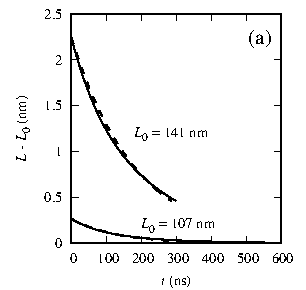
\includegraphics[width=0.32\textwidth]{PermPanelA.pdf}
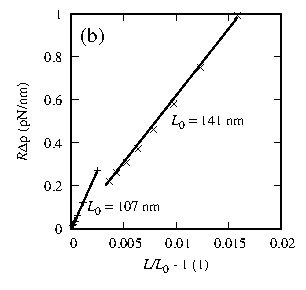
\includegraphics[width=0.32\textwidth]{PermPanelB.pdf}
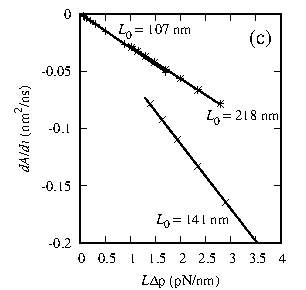
\includegraphics[width=0.32\textwidth]{PermPanelC.pdf}
  \caption{}
    \label{figure:permeability}
\end{figure}

\subsection{Permeability}
Vesicle membranes have a large area modulus $K_A$ and changes in surface are give rise to a membrane tension
$\tilde \gamma = K_A(A/A_0 - 1)$ where $A$ is the membrane surface area and $A_0$ is the reference surface area in the non-tensed state. 
Since we are dealing with two-dimensional vesicles, we replace $A$ and $A_0$ with the membrane arc length $L$ and reference length $L_0$
respectively.  Thus, the tension in a stretched cylindrical vesicle membrane is 
\begin{equation}
\label{eq:stretch}
\tilde \gamma = K_A\left(\frac{L}{L_0} - 1 \right).
\end{equation}
A stretched vesicles has a Laplace pressure 
\begin{equation}
\label{eq:LaplacePressure}
\Delta p = \frac{\tilde \gamma}{R} 
\end{equation}
where $\Delta p$ is the difference in internal pressure to the pressure at infinity
and  $R$ is the radius of the circular vesicle.  The factor 
$R^{-1}$ is the total curvature since  the principle curvature in the direction of the cylinder is zero.

The particles in our setup do not abut but rather have small gaps due to repulsive forces.
The gaps allow for some fluid flux across the JP bilayer.  Aqueous flux is quantified by a permeability constant $P$ in the equation
\begin{equation}
\label{eq:perm}
\frac{dA}{dt} = -P  L \Delta p.
\end{equation}
Combining \eqref{eq:stretch}, \eqref{eq:LaplacePressure}, and \eqref{eq:perm}, we can solve the for length $L$ 
\begin{equation}
\label{eq:perm_solution}
L_0(L-L(0)) + L_0^2 \ln\left|\frac{L-L_0}{L(0)-L_0}\right| = -4\pi^2 P K_A t
\end{equation}
and compare with our data.

Data obtained for the above model.
Case 1. 58 particles with diameter 2.5 nm and $L_0 = 107$ nm. The calculated stretching modulus was $K_A = 109$ pN nm$^{-1}$ which gives 26.5 kT nm$^{-2}$.
This value is in good agreement with the 60 kT nm$^{-2}$ from experimental measurements.  The calculated permeability was 
$0.0296$ nm$^3$ ns$^{-1}$ pN$^{-1}$ = 
$0.0296$ $\mu$m s$^{-1}$ Pa$^{-1}$. (double check value; too large)
Case 2. 117 particles with diameter 1.25 nm and $L_0 = 141$ nm. This data set gave  $K_A = 62$ pN nm$^{-1}$ which gives 15 kT nm$^{-2}$ which is small.
For permeability we get 0.0566 $\mu$m s$^{-1}$ Pa$^{-1}$.

The dashed lines in panel (a) are the graphs of \eqref{eq:perm_solution} for the 58 and 117 particle number cases, respectively. 
Panels (b) and (c) show the select data points with plusses for 58 particles and times for 117 particles.  The solid lines are linear fits.
The linear fits in panel (b) shows that $R\Delta P$ is proportional to relative stretching $L/L_0 - 1$. The proportionality constant is $K_A.$
The linear fits in panel (c) shows that $L\Delta P$ is proportional to flux $\frac{dA}{dt}$.  The proportionality constant is the permeability coefficient $P.$

%\subsection{Jeffery Orbit}
%We use Jeffery orbits to numerically validate our solver for the mobility-problem.  
%The background flow is a shear flow $\uu_{\infty}(\xx) = \dot\gamma  \xx \cdot \mathbf{e}_2 \mathbf{e}_1$ with shear rate $\dot\gamma$
%and orthogonal unit vectors $\mathbf{e}_1$ and $\mathbf{e}_2$. 
%A single elliptical particle is suspended in the fluid with center at the origin.
%The Jeffrey orbit  
%\begin{equation}
%\label{eq:jeff}
%\Theta(t) = \tan^{-1}\left(\frac{a}{b}\tan \left(\frac{ab \dot\gamma t}{a^2+b^2}\right)\right)
%\end{equation}
%gives the angle between the major axis and $\mathbf{e}_2$
%where $a$, $b$ are the semi-major and semi-minor axes. 
%We are assuming $\Theta(0) = 0$.
%Figure~\ref{figure1} shows that the angles coming from the integral equation method \eqref{eq:SKIE}-\eqref{eq:mobility2}
%are in complete agreement with the theoretical time course \eqref{eq:jeff}.  Hydrophobic attraction and repulsion are zero for a single particle. 
%
%
%\begin{figure}
%\centering
%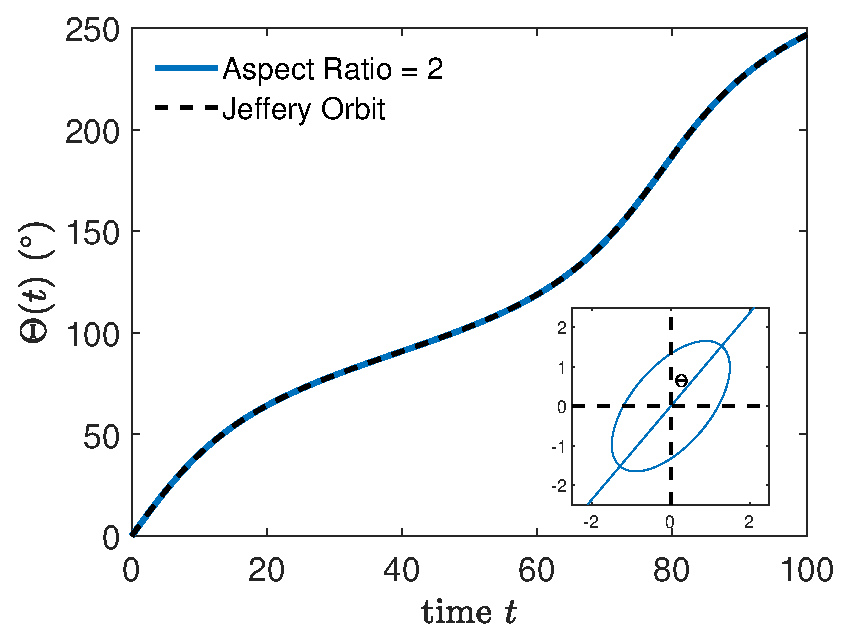
\includegraphics[width=0.4\textwidth]{JefferyOrbit2.eps}
%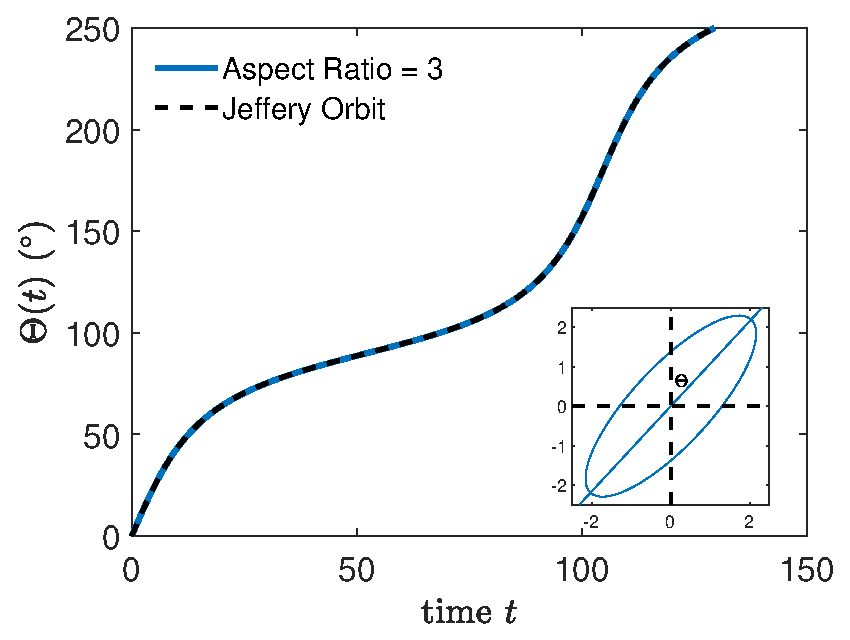
\includegraphics[width=0.4\textwidth]{JefferyOrbit3.eps}
%  \caption{The figure compares the theoretical Jeffery orbit for $\Theta(t)$ and the result from the integral equation method. 
%    The insets show the simulation setup. The shear rate is $\dot\gamma=0.1$.}
%    \label{figure1}
%\end{figure}

%%%%%%%%%%%%%%%%%%%%%%%%%%%%%%%%%%%%%%%%%%%%%%%%%%%%%%%%%%%%%%%%%%%%%%%
\subsection{Self-Assembly and Relaxation}

In order to examine the dynamics of the Janus-vesicle using the HAP coupling with hydrodynamics interactions, for the target bilayer, a circular initial shape is chosen to perform the relaxation run. 
This structure consists of $N=58$ disks with particle radius $r=0.5$ and the starting diameter of 
the vesicle is about $8$ length units.
The starting center of mass position of the Janus-vesicle is pinned at the origin and particle velocities are tracked to determine the initial configuration for later use such as single and multiple vesicle simulations. 
The advantage of acquiring this configuration is to prevent some numerical instability issues when the minimum of the total energy is not achieved. 
For instance, the dynamics of the bilayer under a shear flow may reach different outcomes or equilibrium states.
Figure~\ref{figure2}(a) shows two sets of results: (1) the magnitudes of mean velocity components 
${\bf v}=\{v_x,v_y\}$ decrease exponentially with an approximation decaying rate $\sim0.005$; (2) the variation of the mean particle orientation $\theta$ also decreases over a period of time as expected from the self-assembly property of the model. This implies that a local energy minimum and the equilibrium configuration are nearly attained. 
The time step size $\Delta t=0.2$ is used for all simulations in this work including the relaxation run.
Figure~\ref{figure2}(b) shows the configuration difference between starting and ending frames in the relaxation run. The Figure~\ref{figure2}(c)-(d) demonstrate the fluid pressure profile of two configurations at $t=0$ and $t=1000$. The starting fluid pressure inside the permeable Janus-vesicle decreases as expected.

\begin{figure}
\centering
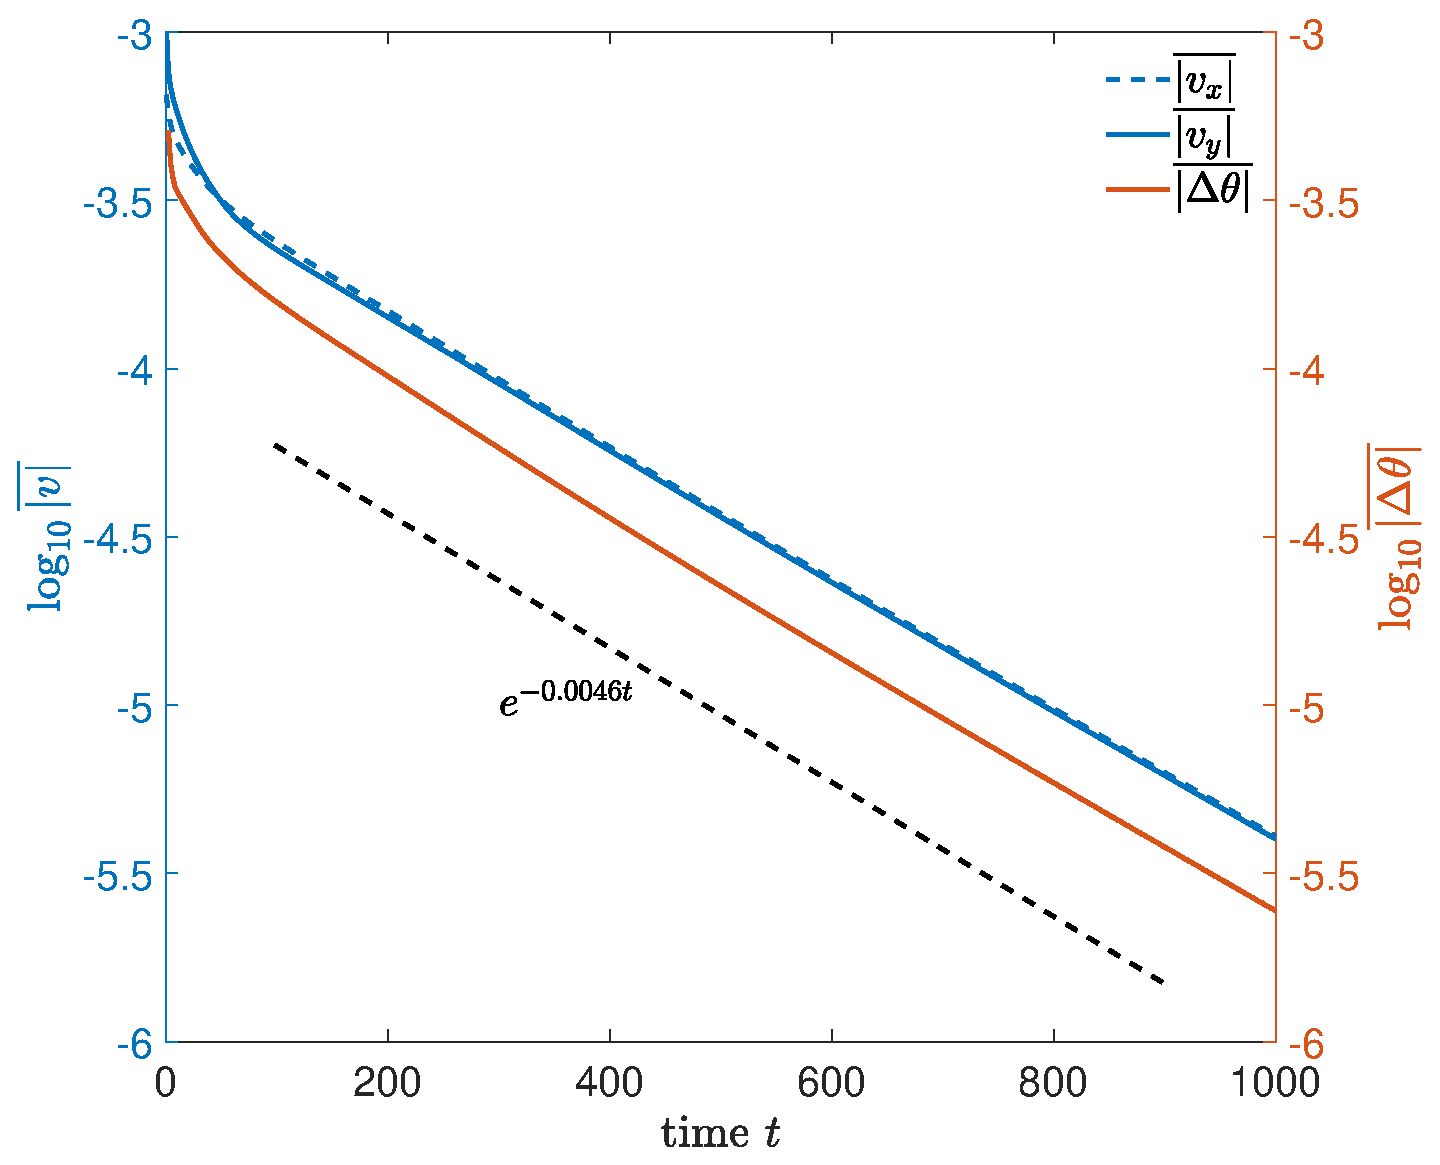
\includegraphics[height=2in]{relax.eps}
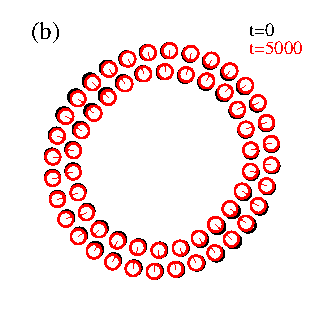
\includegraphics[height=2in]{relax2.eps}\\
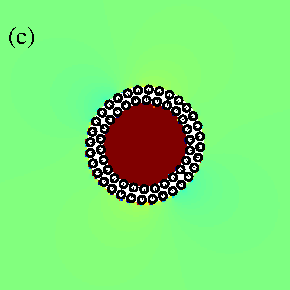
\includegraphics[height=2.in]{N58_0pres.pdf}
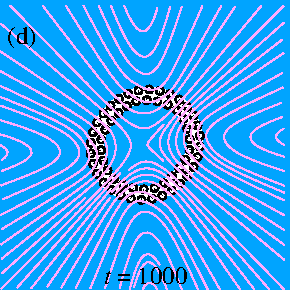
\includegraphics[height=2.in]{N58_5000pres.pdf}
%  \todo[inline]{Put pressure of each of the two configurations below
%  this.}
  \caption{Vesicle relaxes under a quiescent flow. (a) The blue dashed and solid curves are mean magnitudes of the particle velocities in $x$ and $y$ directions, respectively. The red curve shows the decreasing trend of the mean magnitude of particle orientation change. The black dashed line shows the reference of how all magnitudes decay. (b) Bilayer configurations for $t=0$(black) and $t=1000$(red) with particle directors.
  (c)-(d) show the fluid pressure profiles for $t=0$ and $t=1000$ where the background curves indicate the streamlines. In panel (c), the pressure value in internal fluid is much higher than the pressure outside of the bilayer. After the relaxation, this immersed permeable bilayer approaches a steady state as shown in panel (d).
  }
    \label{figure2}
\end{figure}




%%%%%%%%%%%%%%%%%%%%%%%%%%%%%%%%%%%%%%%%%%%%%%%%%%%%%%%%%%%%%%%%%%%%%%%
\section{\label{results}Numerical Results}

%\todo[inline]{Introduce dimensionless shear rate here (and check the numbers)}

Following the relaxation experiments we consider the behavior of
Janus-vesicles under various flows. To extract physical quantities of
the target structure, we introduce the following scaling laws and the
dimensionless units. The length unit is scaled by the length of
phospholipids $l=2.5$~nm which is the diameter of each Janus particle.
The force is scaled by the interfacial tension $\gamma=4.11$~pN
nm$^{-1}$ from~\cite{Ryham16}. This means that the energy unit is scaled
by $1\ k_BT$. We can then define the characteristic time scale $\tau =
\mu l/\gamma = 0.61$~ns where the fluid viscosity is $\mu=1$ cP.  With
the same framework,~\cite{Fu20} provide the bending rigidity
$\kappa=8.51$~$k_BT$. For the model parameters, the decay length of
attraction is $\rho = 2l = 5$~nm, the repulsion length scale is
$\rho_0=0.5$, and the repulsion strength is $M=4.0$~$k_BT$. Finally, the
dimensionless shear rate is $\chi = \dot\gamma \tau$ where $\dot\gamma$
is the shear rate.


%For the $N$-body Janus-vesicle, we denote a constant initial radius $R_0=\sqrt{A_0/4\pi}$ with initial area $A_0$

%referred from~\cite{Finken08} and~\cite{Shaqfeh11},
%\begin{align}
%  \chi = \dot\gamma \frac{\mu R_0^3}{\kappa},
%\end{align}
%%
%where $\dot\gamma$ the dimensional shear rate, and $\mu$ the fluid viscosity.


%%%%%%%%%%%%%%%%%%%%%%%%%%%%%%%%%%%%%%%%%%%%%%%%%%%%%%%%%%%%%%%%%%%%%%%
\subsection{Tank-Treading Vesicles}

%%%%%%%%%%%%%%%%%%%%%%%%%%%%%%%%%%%%%%%%%%%%%%%%%%%%%%%%%%%%%%%%%%%%%%%
\subsubsection{Vesicle in a Shear Flow}
\label{sec:ves_in_shear}
We begin by studying the dynamics of a single Janus-vesicle suspended in
the shear flow
\begin{align}
  \uu_{\infty}(\xx) = \dot\gamma (\xx \cdot \mathbf{e}_2) \mathbf{e}_1,
\end{align}
with shear rate $\dot\gamma$, and orthogonal unit vectors $\mathbf{e}_1$
and $\mathbf{e}_2$ for the horizontal and vertical directions
respectively. It is well known that a vesicle has tank-treading behavior
when there is no viscosity contrast between the fluids inside and
outside of the vesicle.
%Within the framework of the simulation setup,
%the proposed model provides a feature that the fluid viscosity is
%constant over the computational domain and it is capable of performing
%these simulations.

The centroid of the pre-relaxed $58$-body Janus vesicle is initially
placed at the origin and the shear flow with a certain shear rate $\chi$
is applied. Snapshots of the Janus-vesicle in a shear flow with a shear
rate $\chi=0.0025$ are shown in Figure~\ref{figure3}. Panels (a) and (b)
show the initial shape obtained from the relaxation run and the deformed
configurations of the Janus-vesicle at time $t=4000$ are in panels (c)
and (d). The background color in panels (a) and (c) is the strength of
the action of the hydrophobic attraction. Red corresponds to a strong
action while blue is weak action. The hydrophobic layer clearly has the
strongest action. To demonstrate the tank-treading behavior of the
vesicle, panels (b) and (d) provide the streamlines of the fluid
velocity around the Janus-vesicle. In panel (d), we can clearly observe
the clockwise tank-treading motion.


\begin{figure}
\centering
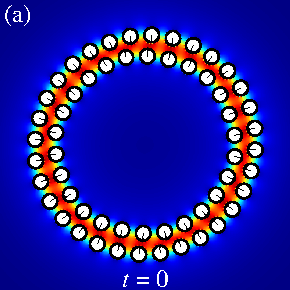
\includegraphics[width=0.3\textwidth]{N58_0.pdf}
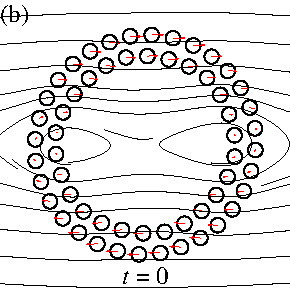
\includegraphics[width=0.3\textwidth]{N58_vel_0.pdf}\\
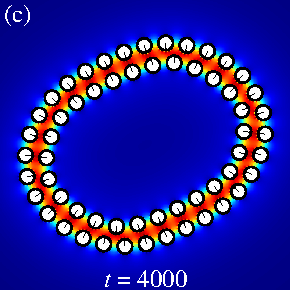
\includegraphics[width=0.3\textwidth]{N58_20000.pdf}
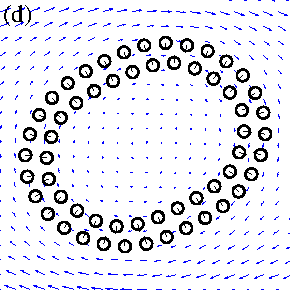
\includegraphics[width=0.3\textwidth]{N58_vel_20000.pdf}
  \caption{\label{figure3} A Janus-vesicle suspended in a shear flow
  with shear rate $\chi=0.0025$: (a) Initial configuration of 58-body
  Janus-vesicle where black arrows are the particle orientations. (b)
  The particle velocities and streamlines of the configuration in (a).
  Streamlines are plotted in the background as solid curves. Red arrows
  represent the particle velocities. (c) Deformed Janus-vesicle at
  $t=4000$. At this configuration the Janus-vesicle is tank-treading.
  (d) The particle velocities and streamlines of the configuration in
  (c). The background colors in panels (a) and (c) represent the
  strength of the hydrophobic attraction potential. The blue region
  shows no action and the red region in the bilayer gives the strongest
  action.}
\end{figure}
%
%

To extract additional physical properties of the proposed model, we
compute the total length, reduced area, and excess length of the bilayer
structure. The enclosed area and the total length of the structure are
calculated from the midplane. The reduced area is $A^* = 4\pi A/L^2$
where $A$ the area, and $L$ the total length of the Janus-vesicle, and
the excess length is $\Delta=L/\sqrt{A^*/\pi}-2\pi$.
Figure~\ref{figure4} shows these quantities for a Janus-vesicle
suspended in a shear flow with shear rates
$\chi=\{0.002,0.0025,0.003,0.0035\}$. Since the starting configuration
is nearly circular, the reduced area decreases from an initial value
close to $1$. The smooth curves in panel (a) are best fits of the
exponential model $A^* = a_0 + b_0 \exp(-kt)$. Panel (b) shows that the
decay rate $k$ is independent of the shear rate for sufficiently large
shear rates, and the terminal reduced areas of each case are shown in
the inset. We see that lower shear rates generate a higher final reduced
area. In particular, we observe that the reduce area converges
relatively early when the shear rate is lower than $\chi=0.003$. 
%and has a faster convergence than the high shear rate cases.
Panel (c) shows that the total arc length remains constant for all time
with all four shear rates. Combining the behavior of the reduced area
and the total arc length, the excess length must increase in time and be
larger for higher shear rates as observed in panel (d). In all these
results, there are oscillations that can be explained by the granularity
of the Janus-vesicle which results in a midplane that is non-smooth.
%Overall the total lengths of the bilayer have the same converging value
%in all test shear rates.

\begin{figure}
\begin{center}
\hspace{-0.6cm}
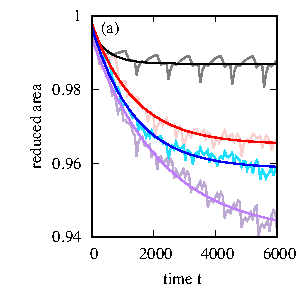
\includegraphics[height=2in]{ReducedArea.pdf}
\hspace{0.6cm}
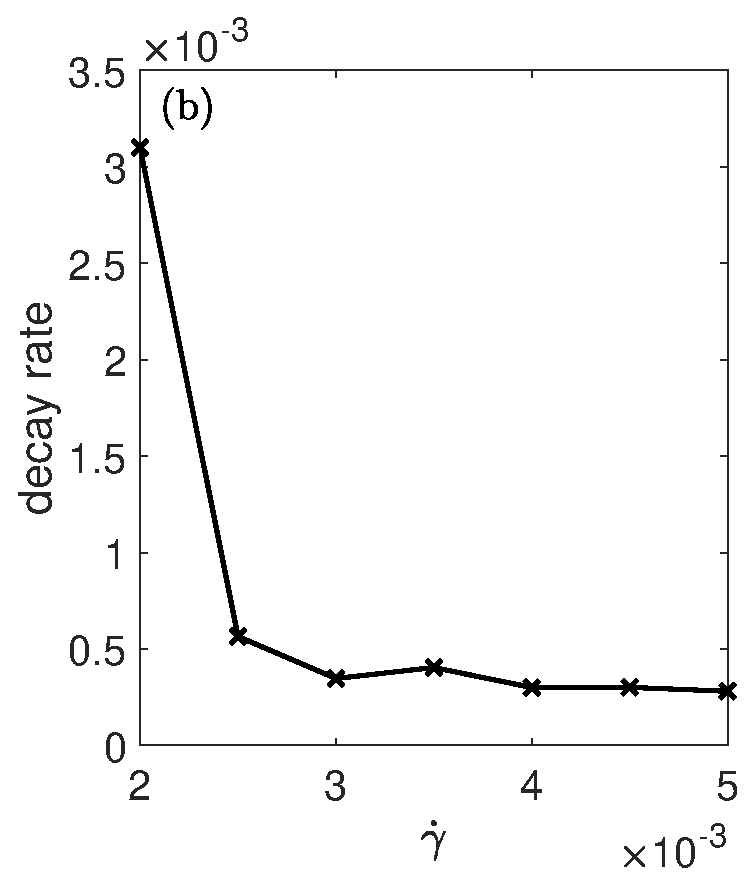
\includegraphics[height=2in]{DecayRate.eps}\\
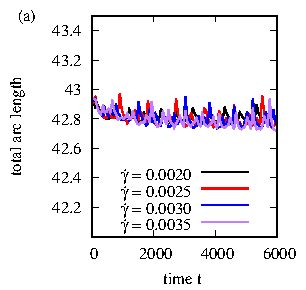
\includegraphics[height=2in]{ArcLength.pdf}
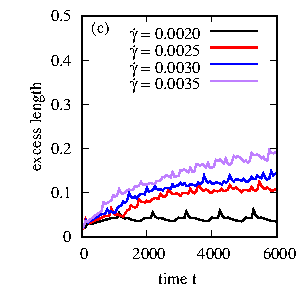
\includegraphics[height=2in]{ExcLength.pdf}
\end{center} 
  \caption{\label{figure4} (a) Total arc lengths of the midplanes over
  time for four shear rates. (b) From exponential fits in panel (a), we
  obtain the decay rate $k$ for a number of different shear rates. The
  inset plots the terminal reduced areas. (c) Reduced area transitions
  over time. (d) Excess length of the midplanes. For all panels, a set
  of shear rates $\chi=\{0.002,0.0025,0.003,0.0035\}$ is used in
  simulations. The legend in panel (d) applies to both panels (a) and
  (c).}
\end{figure}




\subsubsection{Intermonolayer friction}
An interesting phenomenon also rises up in the proposed setup where the inter-monolayer slip occurs 
between two leaflets. When a shear rate is large enough, take $\chi = 0.005$ as an example, 
Figure~\ref{figure5} shows the schematic of the test where a particle pair is initially marked and we then track the positions of this particle pair over a period of time. 
In this series of tests, we monitor the mean particle position change and mean angle $\theta(t)$ between particle relative positions with respect to the vesicle center over the time. It is clear to see that the outer leaflet always has larger tangential velocity than the one from the inner leaflet and the mean angle $\theta(t)$ increases. This inter-leaflet sliding phenomenon is consistent with what has been seen
in articles in molecular dynamics simulations.

%
%\todo[inline]{Figure/Table of the friction coefficient for different shear rates (needs to revise)}


\begin{figure}
\begin{center}
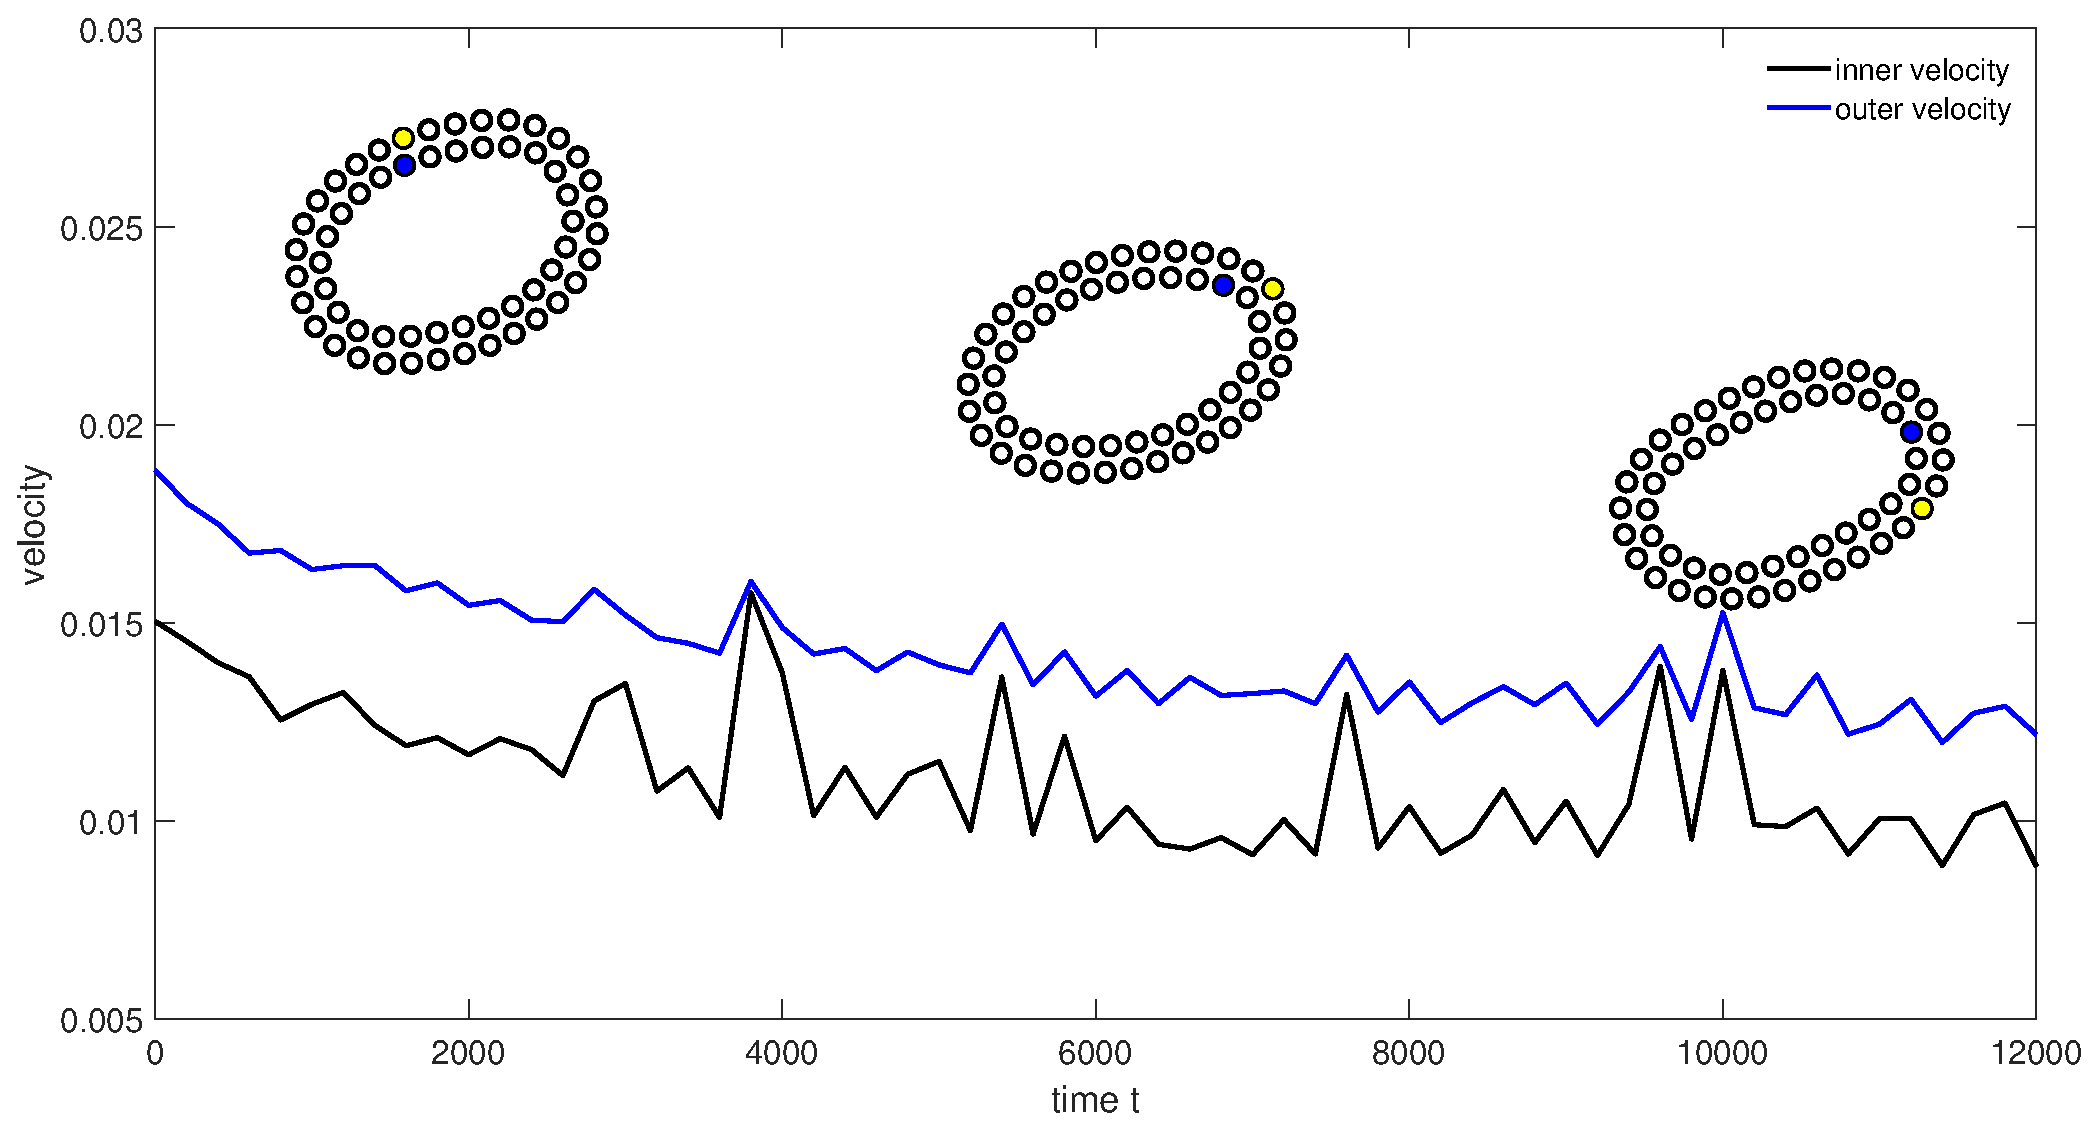
\includegraphics[width=0.5\textwidth]{Slip.eps}
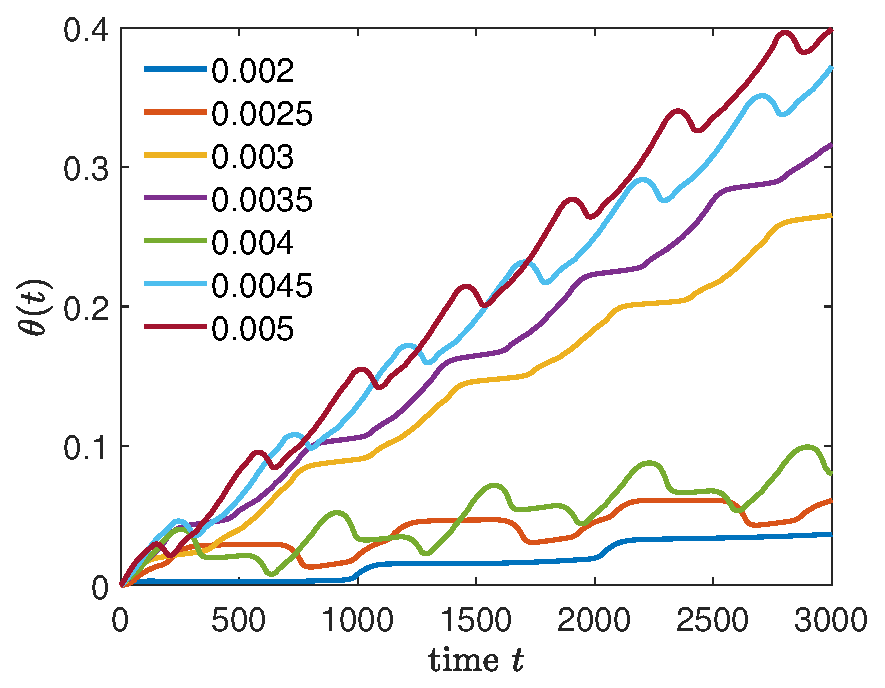
\includegraphics[width=0.4\textwidth]{Slip2.eps}
\end{center} 
  \caption{The schematic of the intermonolayer slip over a period of time. Taking shear rate $\chi=0.005$ as an example, we denote the mean angle between each particle pair $\theta(t)$ where the angle is calculated from the relative position of particles using the vesicle center of mass position. The configuration plots have two fixed particles marked in yellow and blue and labeled with the corresponding time $t=2000$ and $t=9000$. The midplane curve is denoted as $\Sigma_M$. We provide numerical results of $\theta(t)$ for cases of shear rates $\chi$.
  }
    \label{figure5}
\end{figure}



To calculate the inter-monolayer friction coefficient for the apposing JP leaflets, we let  
\begin{equation}
b = \frac{\langle F\rangle}{\langle L \rangle \langle U\rangle },
\end{equation}
%
where $\langle F\rangle = \langle \int_{\mathcal{C}_M} \jump{\ttau \cdot \sigma \cdot \nnu} \,ds\rangle$ 
is the time-averaged, tangential force along the midplane curve $\mathcal{C}_m$. 
The parameters $\langle L\rangle$ and $\langle U\rangle$ are the time-averaged midplane curve length and
intermonolayer slip velocity respectively.  

We calculate $\langle F\rangle$ by first evaluating the smooth tangential force along curves a positive distance inside and 
outside $\mathcal{C}_m$ respectively, and then interpolating at zero distance to give a force jump. 
We have made a slight abuse of language: due to the problem being two-dimensional,
the integral $\langle F\rangle$ is actually a force density per length which when divided by length gives the requisite force per area. 
%which when divided by length 

Table~\ref{table1} provides dimensional friction coefficients $b$ for several shear rates
and the results are in quantitative agreement with 
values previously reported in the literature~\cite{sch-vla-mik2010} and~\cite{denOtter2007}.  
The coefficients generally lie within the range 0.2 to 0.3 pN$\cdot$ns nm$^{-3}$ but there are some 
outliers.  These outliers ($\dot\gamma = 0.0041$ ns$^{-1}$ and 
$\dot\gamma = 0.0066$ ns$^{-1}$) correspond to slip velocities that are too low relative to shear rate (see the green and red curve in Figure \ref{figure5}: panel (c)).
The JP vesicle consists of only  58 particles and so it is not surprising that discrete effects produce outliers. 

\todo[inline]{If $B$ is the numerically calculated friction coefficient,  then 
$b = B/2.5^3$ pN ns nm$^{-3}$ gives the dimensional value.

If $P$ is the numerically calculated pressure, then $p = P/2.5$ pN nm$^{-2}$ is the dimensional pressure.} 

\begin{table}
\caption{Friction Coefficients}
\centering    
\begin{tabular}{c c c c c c c c }
 $\chi$ & 0.0020   &  0.0025 &  0.0030 &  0.0035 &  0.0040 & 0.0045 & 0.0050  \\
\hline                    
$\dot\gamma$ (ns$^{-1}$)        & 0.0033 & 0.0041 & 0.0049 & 0.0057 & 0.0066 & 0.0074 & 0.0082\\
%$F_{f}$ (pN nm$^{-1}$)           & 1.84 & 4.90 & 11.36 & 8.16 & 6.14 &  17.69 &  24.33 \\[1ex]
%$\dot\theta$ (nm ns$^{-1}$)           & $6.84\times10^{-5}$ & $1.31\times10^{-4}$ & $3.46\times10^{-4}$ & $2.32\times10^{-4}$ & $1.81\times10^{-4}$ & $4.91\times10^{-4}$ & $5.83\times10^{-4}$\\ [1ex]
$b$ (pN$\cdot$ns nm$^{-3}$)    & 0.22 & 0.87  & 0.22 &0.21 & 1.29 & 0.31 & 0.30\\ 
\hline    
\end{tabular} 
\label{table1}
\end{table}


%%%%%%%%%%%%%%%%%%%%%%%%%%%%%%%%%%%%%%%%%%%%%%%%%%%%%%%%%%%%%%%%%%%%%%%
\subsubsection{Vesicle in a Parabolic Flow}

Besides the tests of a Janus-vesicle in a shear flow, an interesting test can also use the proposed model and the setup. Consider a symmetric parabolic flow about the $x$-axis, \cite{Kaoui09} studied shapes of the red blood cell immersed in a parabolic flow using a continuum model. With a similar setup, the background flow for this set of simulations is given by
\begin{equation}
\uu_\infty = v_{max}\left[ 1 - \left( \frac{y}{wR_0}\right)^2 \right]{\bf e}_x,
\end{equation}
%
where $v_{max}$ is the flow strength and $w$ controls the shape of the flow. $R_0$ is defined as the radius of the Janus-vesicle at $t=0$. 

Figure~\ref{figure6} gives three configurations for one specific case where the centroid of the Janus-vesicle is initially placed slightly above the $x$-axis. The parameters are $v_{max} = 8.0$, $w=10$, and $R_0=8$. The red curves are the midplanes and a particle pair is marked in color. We observe that the deformed 
Janus-vesicle has a counterclockwise movement and the shape of the vesicle approaches to an asymmetric
slipper shape. For this test run, the reduced area for this configuration is $\sim0.9$ which matches the previous numerical tests in \cite{Kaoui09} where a slipper-like shape occurs when the flow velocity is weak and the reduced area is large. 
A schematic of the setup is shown in Figure~\ref{figure7} where the blue horizontal line represents the mean
$y$-position of all particles. The inset of Figure~\ref{figure7} shows the trajectory of the mean position in 
$y$-direction which decreases toward $y=1$ for a period of time and starts to have an oscillatory motion. 


\begin{figure}
\centering
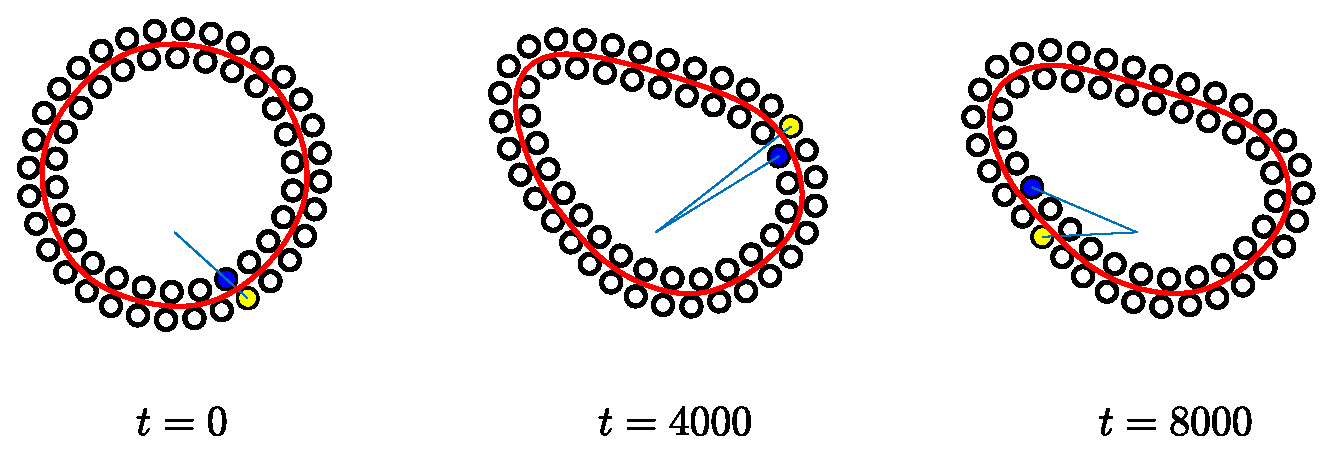
\includegraphics[width=0.8\textwidth]{slipper.eps}
  \caption{Vesicle under a parabolic flow where the strength of the flow $v_{max}=32.8$ nm ns$^{-1}$, $R_0 = 20$ nm,  and the control parameter $w=10$. The configuration is the state when $t=\{0, 4000, 8000\}$. Red curves are midplanes of three configurations. 
  }
    \label{figure6}
\end{figure}


\begin{figure}
\centering
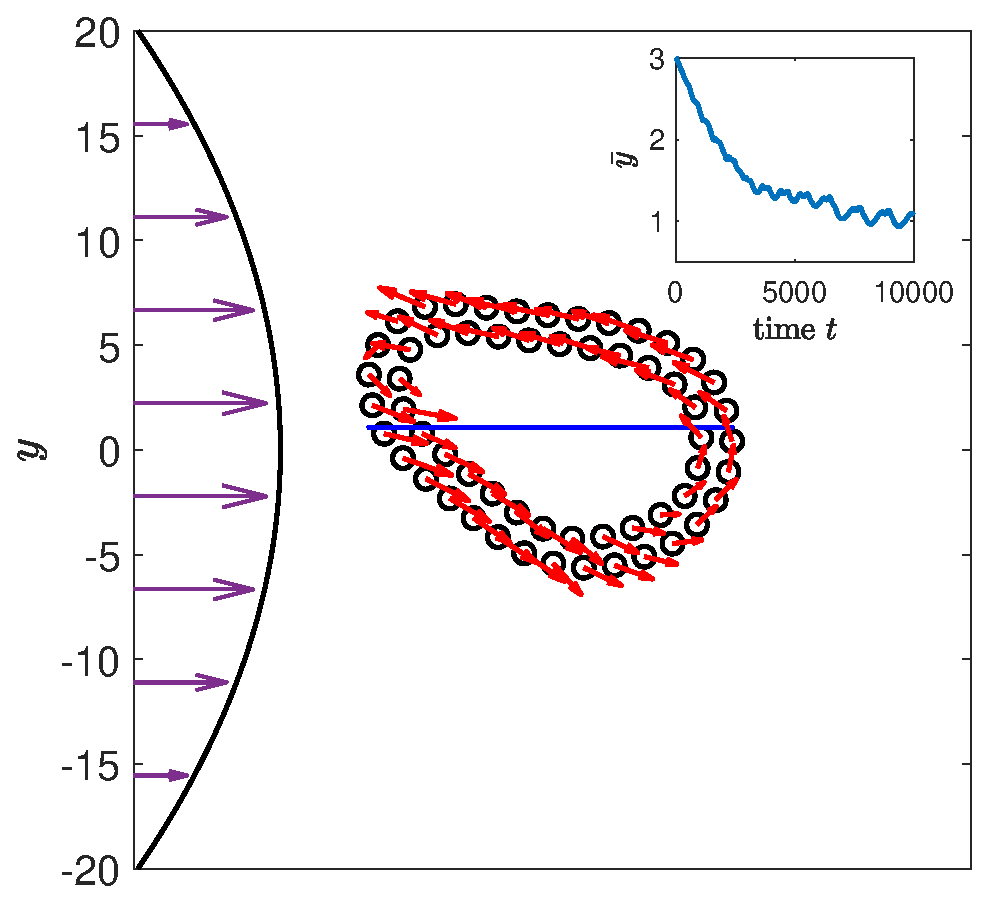
\includegraphics[height=2in]{parabolic.eps}
  \caption{Schematic of a Janus-vesicle under a parabolic flow where the strength of the flow $v_{max}=32.8$ nm ns$^{-1}$, $R_0 = 20$ nm,  and the control parameter $w=10$. The configuration is generated when $t=10000$. The inset plots the trajectory of mean $y$-position over the time.
  }
    \label{figure7}
\end{figure}




%%%%%%%%%%%%%%%%%%%%%%%%%%%%%%%%%%%%%%%%%%%%%%%%%%%%%%%%%%%%%%%%%%%%%%%
\subsubsection{Membrane Ruptures}


With the choice of a large shear rate, a pore formation or a complete membrane rupture can be captured during simulations. Figure~\ref{figure8} shows a demonstration of a vesicle under a shear flow with shear rate $\chi=0.1$. An interesting phenomenon occurs in panels (c) and (d) where two separated bilayers move along the background shear flow symmetrically. Consequently, a periodic motion for bilayers may occur 
with the choices of shear rates. One can expect that these two layers will flow far apart from each other for much higher shear rates.



\begin{figure}
\centering
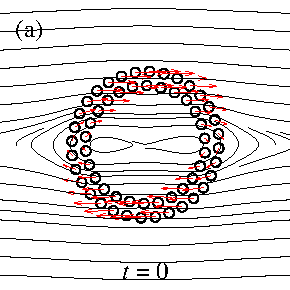
\includegraphics[height=2in]{N58_rupt_0.pdf}
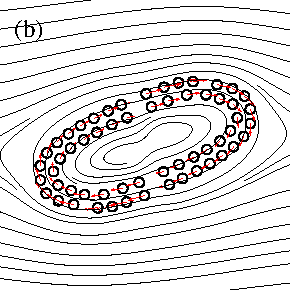
\includegraphics[height=2in]{N58_rupt_200.pdf}
\\
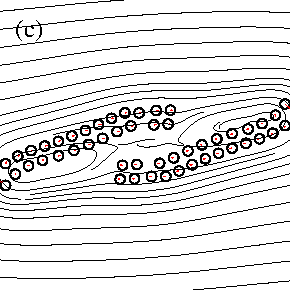
\includegraphics[height=2in]{N58_rupt_400.pdf}
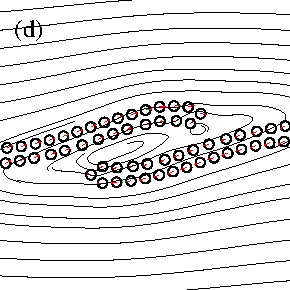
\includegraphics[height=2in]{N58_rupt_600.pdf}
  \caption{Membrane rupture occurs when the shear rate is beyond a certain threshold. Here the shear rate is $\chi = 0.1$. Starting with a circular shape (panel (a)), the vesicle is stretched by the background flow and multiple pores appear (panel (b)). (c)-(d) are the later states during the simulation.
  }
    \label{figure8}
\end{figure}




%%%%%%%%%%%%%%%%%%%%%%%%%%%%%%%%%%%%%%%%%%%%%%%%%%%%%%%%%%%%%%%%%%%%%%%
\subsection{Two Vesicles in a Linear Flow}


\begin{figure}
\begin{center}
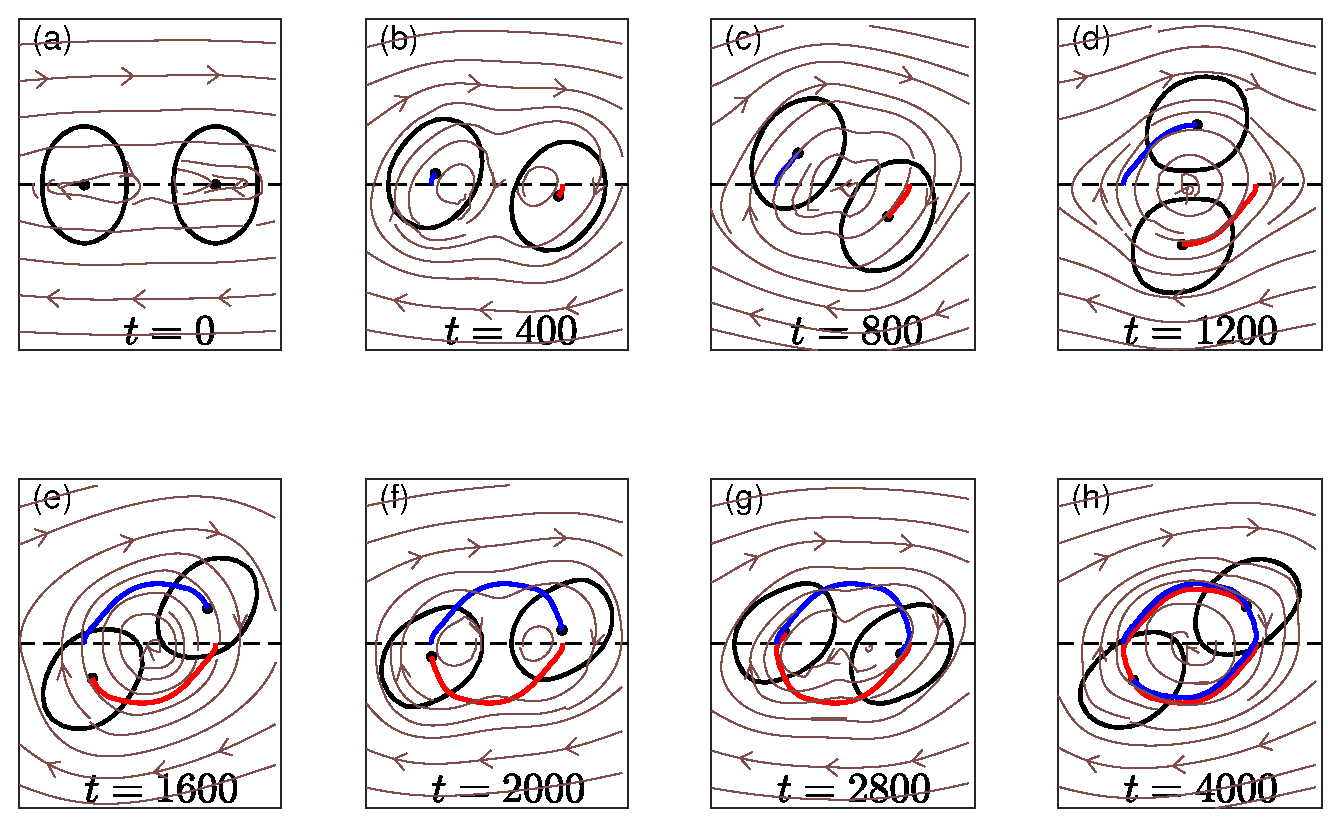
\includegraphics[width=0.9\textwidth]{ShearTraj.eps}
\end{center} 
  \caption{Trajectories of two-vesicle in a shear flow. The moving paths of two centroids of two Janus-vesicles are plotted in blue and red. Both starting centroids of two Janus-vesicles are on the $x$-axis. 
For simulation time, $t = {0, 400,800,1200}$ for (a)-(d) and $t = {1600, 2400, 3200, 4000}$ for (e)-(h).}
    \label{figure9}
\end{figure}

\begin{figure}
\centering
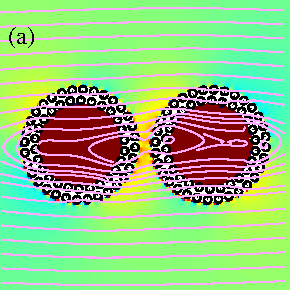
\includegraphics[height=2in]{N116_shear_0.pdf}
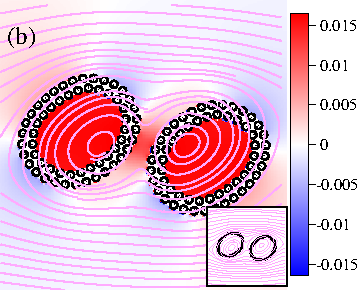
\includegraphics[height=2in]{N116_shear_2500.pdf}\\
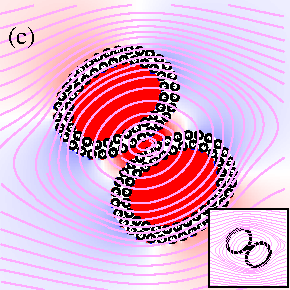
\includegraphics[height=2in]{N116_shear_5000.pdf}
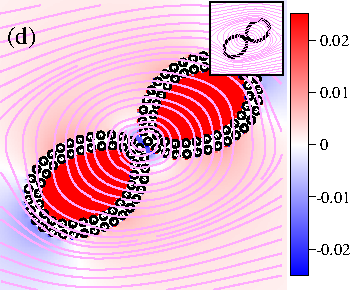
\includegraphics[height=2in]{N116_shear_7500.pdf}
  \caption{Two vesicles under a shear flow where the dimensioneless shear rate is $\chi=0.005$; The initial configuration is shown in panel (a). The background color indicates the magnitude of fluid pressure. From dark red to dark blue, it represents the the pressure varies from high to low values. The color bar is valid for all panels. Streamlines are plotted in purple. The insets of all panels are generated from the results of continuum modeling simulations and the streamlines have a perfect agreement to the numerical results.
  }
    \label{figure10}
\end{figure}




%%%%%%%%%%%%%%%%%%%%%%%%%%%%%%%%%%%%%%%%%%%%%%%%%%%%%%%%%%%%%%%%%%%%%%%
\subsubsection{Shear Flow}


Figure~\ref{figure9} demonstrates the simulation results of two Janus-vesicles in a shear flow where the testing shear rate is $\chi=0.005$ and the flow is given by $\dot x = \chi y$. 
In panel (a), the starting frame, two center-of-mass positions are placed 
on the same horizontal level, at $(-10,0)$ and $(10,0)$. Since we already have a pre-relaxed $58$-body in previous sections, we duplicate the state to have the initial configuration (shown in panel (a)) in this section. 
In all panels, the blue and red curves represent the moving paths of two Janus-vesicle centroids and they move nearly a round when $t=4000$ as shown in panel (h). 
We observe that the rotation continues as time goes and an interesting event occurs in the simulation that an adhesive effect can be seen and tuned. In other words, the adhesive behavior will be absent when two vesicles are centered at a different level and are well separated in $y$-direction. 

The fluid pressure profiles of snapshots are given in Figure~\ref{figure10}.
As expected, there is no pressure jump between the internal and external fluids from the beginning of the
simulation and this is shown in the background pressure plot. 
Panels (b)-(d) show the configurations when $t = \{500,1000,1500\}$ and 
the streamlines are plotted in the background for all panels. We include the numerical results using 
a continuum model in all insets and these comparisons give a qualitative agreement between two models.


%\todo[inline]{Migration pattern and/or separation distance. See Fig 8 in
%JCP paper by Rahimian, Veerapaneni, and Biros.}



\begin{figure}
\begin{center}
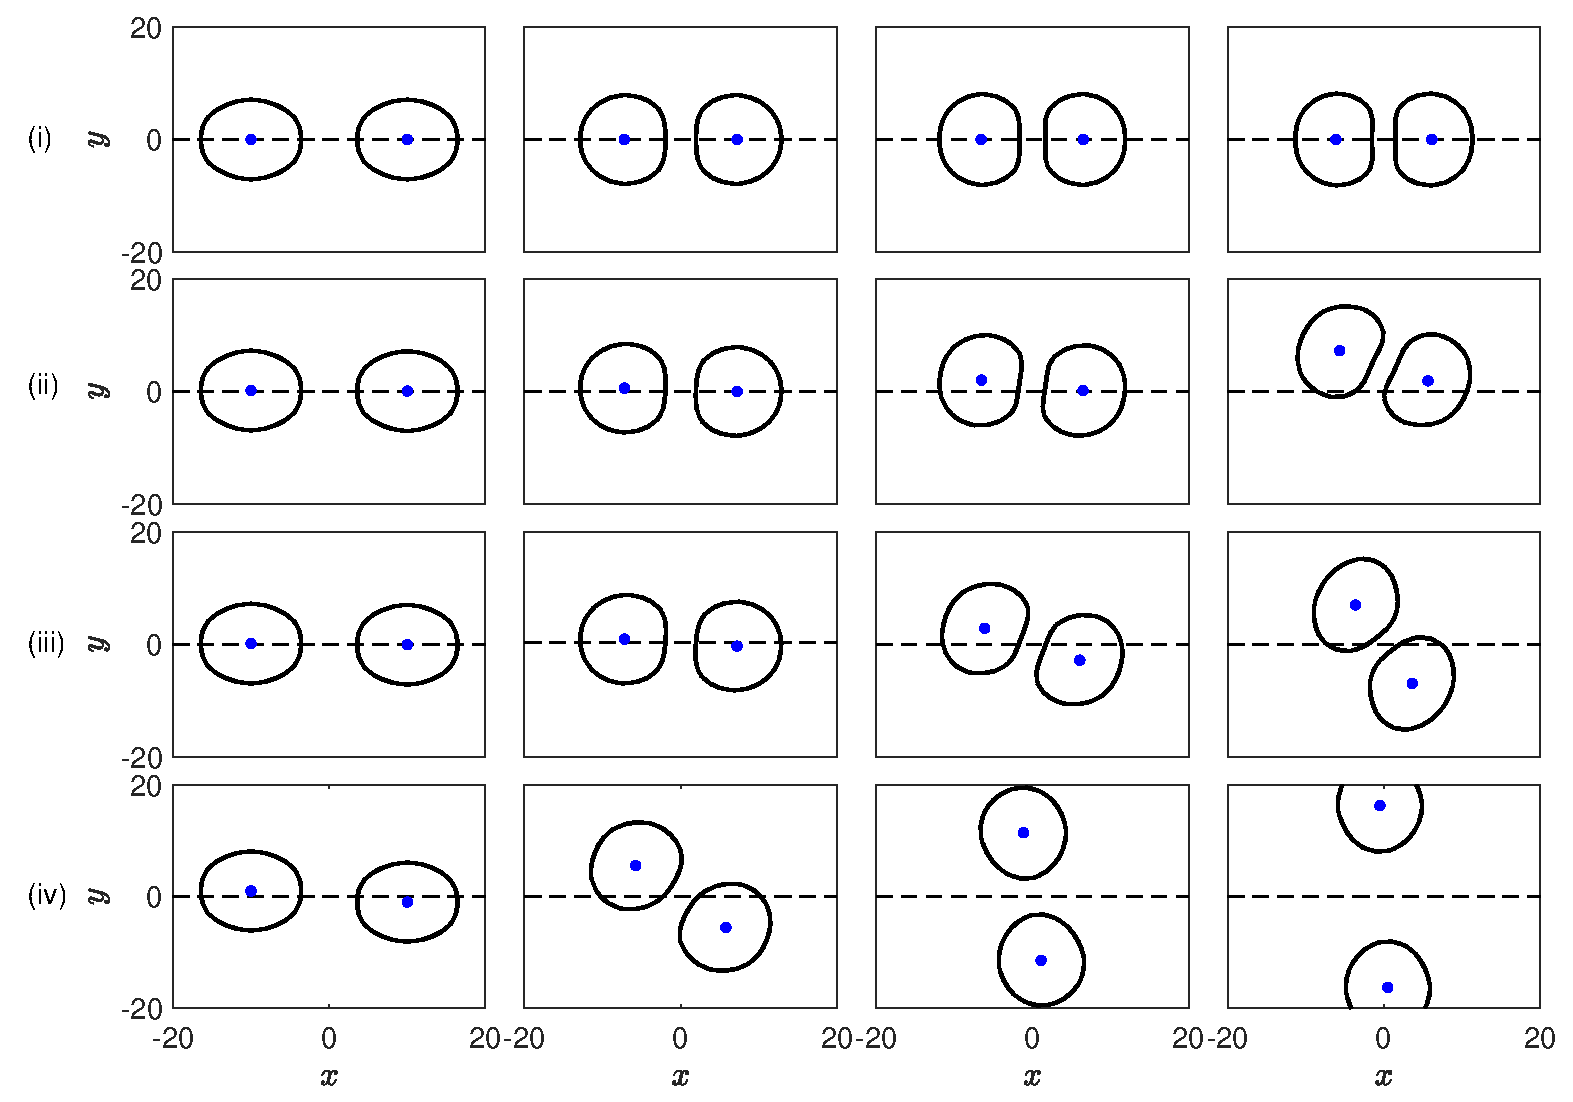
\includegraphics[width=0.9\textwidth]{ExtTraj.eps}
\end{center} 
  \caption{Trajectories of different setups in two-vesicle in an extensional flow and the moving paths of two centroids of two Janus-vesicles are plotted in blue and red. (i) Both centroids of two Janus-vesicles are on the $x$-axis; (ii) The centroid of the left Janus-vesicle is $0.1$ unit above the $x$-axis; (iii) 
  The centroid of the left Janus-vesicle is $0.1$ unit above the $x$-axis and the other one is $0.1$ unit below the $x$-axis; (iv) The centroid of the left Janus-vesicle is $0.5$ unit above the $x$-axis and the other one is $0.5$ unit below the $x$-axis; Figure~\ref{figure12} presents the numerical results from the case (iii) and a 
  consistent flow rate is $\chi = 0.005$ for all cases.}
    \label{figure11}
\end{figure}


\begin{figure}
\centering
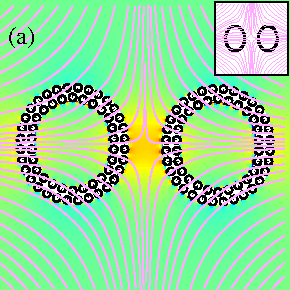
\includegraphics[height=2in]{N116_ext_0.pdf}
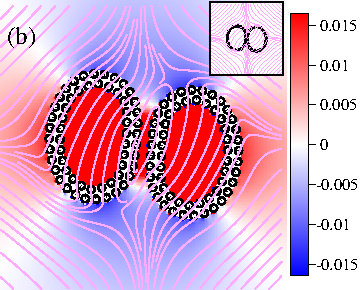
\includegraphics[height=2in]{N116_ext_2000.pdf}\\
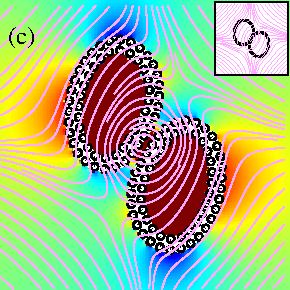
\includegraphics[height=2in]{N116_ext_4000.pdf}
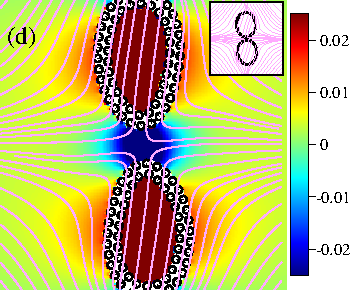
\includegraphics[height=2in]{N116_ext_6500.pdf}
  \caption{Two vesicles under an extensional flow where the dimensioneless shear rate is $\chi=0.005$; The initial configuration is shown in panel (a). The background color indicates the magnitude of fluid pressure. From dark red to dark blue, it represents the the pressure varies from high to low values. The color bar is valid for all panels. Streamlines are plotted in purple. The insets show the results produced from using continuum model that the streamlines have perfect agreements with the present results.
  }
    \label{figure12}
\end{figure}





%%%%%%%%%%%%%%%%%%%%%%%%%%%%%%%%%%%%%%%%%%%%%%%%%%%%%%%%%%%%%%%%%%%%%%%
\subsubsection{Extensional Flow}


With a similar setup in the case of two Janus-vesicles in a shear flow, we use the same two pre-relaxed $58$-body Janus-vesicles to perform the simulations when the flow type is an extensional flow with flow rate $\chi=0.005$. This extensional flow is stretching along the $y$ direction and squeezing in $x$ direction.
Figure~\ref{figure11} provides simulation results when the center-of-mass positions are placed differently.
One can notice that when two centroids are placed on the same horizontal level, two Janus-vesicles reach
an equilibrium state without separation as shown in case (i). If only one centroid is placed above the $x$-axis, for instance, case (ii), two Janus-vesicle move together toward the upward. This is the consequence when the adhesive effect beats the flow strength. In case (iii), two centroids have a small bias in $y$-direction and they
start to move apart along $\pm y$-direction. Finally, case (iv) has a larger initial separation in $y$-direction and two Janus-vesicle moves much faster toward $\pm y$-directions.

Figure~\ref{figure12} shows numerical results when the centroids of two bodies are placed at
$(-10,-0.1)$ and $(10,0.1)$, that is, case (iii) of Figure~\ref{figure11}. With this setup, 
we can make sure that two Janus-vesicles will separate along $y$-direction eventually and we compare the results against a continuum model as shown in all insets. 
Panels (b)-(d) show the transitions of two vesicles moving under an extensional flow.  Since two bilayers are close enough from the beginning of the run, two vesicles are first pushed toward each other then separate along the streamlines. In fluid pressure profiles, the pressure is initially high between the gap formed by two 
Janus-vesicles and decreases during the separation. The short range repulsion plays an important role to avoid structure collisions and this result can be compared with some findings in continuum modeling simulations. 


%may need to add more here


%\todo[inline]{Make figure of the paths of the two centroids....}



%%%%%%%%%%%%%%%%%%%%%%%%%%%%%%%%%%%%%%%%%%%%%%%%%%%%%%%%%%%%%%%%%%%%%%%
\section{\label{conclusion}Conclusion}




This study proposes a continuum coarse-grained model for Janus-vesicle that focuses on the 
hydrophobic interactions between lipids and hydrodynamic interactions.
The mobility problem using integral equation methods combines the previously introduced HAP and the 
revised hydrophobic force for obtaining particle dynamics. 
The imposed forces and torques of Janus particles adopt not only HAP but a newly developed short 
range repulsion given by \ref{eq:REPULforce} and \ref{eq:REPULtorque}.
The hydrodynamic stress tensor calculated in the algorithm leads to examinations of permeable 
membrane where the stretching modulus $K_A$ and the permeability constant $P$ can be obtained.


With the use of selected parameters, the numerical algorithm yields good qualitative results such as
phenomena in tank-treading Janus-vesicle and asymmetric slipper shape in a parabolic flow. 
We also demonstrate the membrane rupture in a flow at high shear rate and this makes a breakthrough 
about having an idea for simulating such phenomenon different from other continuum modeling simulations.
Inter-monolayer friction coefficients are then obtained and reported by calculating the pressure jumps and
slip velocities with respect to the bilayer midplane.
Results of two Janus-vesicles in flow simulations produce an outstanding agreement with ones generated 
using continuum modeling.

Our future goal is to extend the current framework to a three-dimensional Janus-vesicle system. 
The further implementation of adding a fast algorithms such as the fast multipole method is also a 
practical approach.







\begin{acknowledgments}
%We would like to acknowledge 
\end{acknowledgments}

\appendix

\section{Appendices}
\label{sec:appendixA}

\bibliographystyle{jfm}
\bibliography{reference}% Produces the bibliography via BibTeX.





%\bibliographystyle{jfm}
%\bibliography{jfm}
%Use of the above commands will create a bibliography using the .bib file. Shown below is a bibliography built from individual items.


%\bibliography{jfm2esam}

%\begin{thebibliography}{99}
%
%\expandafter\ifx\csname natexlab\endcsname\relax
%\def\natexlab#1{#1}\fi
%\expandafter\ifx\csname selectlanguage\endcsname\relax
%\def\selectlanguage#1{\relax}\fi
%
%\bibitem[Batchelor (1971)]{Batchelor59}
%{\sc Batchelor, G.K.} 1971 {Small-scale variation of convected quantities like temperature in turbulent fluid part1, general discussion and the case of small conductivity}, {\it J. Fluid Mech.}, {\bf 5}, pp. 3-113-133.
%
%\bibitem [Bouguet (2008)]{Bouguet01}
%{\sc Bouguet, J.-Y} 2008 Camera Calibration Toolbox for Matlab {\url{http://www.vision.caltech.edu/bouguetj/calib_doc/}}.
%
% \bibitem[Briukhanovetal et al (1967)] {Briukhanovetal1967}
%{\sc Briukhanov, A. V.,   Grigorian, S. S., Miagkov,  S. M., Plam, M. Y.,   I. E. Shurova, I. E.,   Eglit, M. E. and Yakimov, Y. L.} 1967
%{On some new approaches to the dynamics of snow avalanches},
%{\it Physics of Snow and Ice,  Proceedings of the International Conference on Low Temperature Science}
%{Vol 1} pp. 1221--1241 {Institute of Low Temperature Science, Hokkaido University, Sapporo, Hokkaido, Japan}.
%
%\bibitem[Brownell (2004)]{Brownell04}
% {\sc Brownell,  C.J.  and Su,  L.K.} 2004  {Planar measurements of differential diffusion in turbulent jets}, {\it AIAA Paper},  pp. 2004-2335.
%
%\bibitem[Brownell and Su (2007)] {Brownell07}
%  {\sc Brownell, C.J. and  Su, L.K.} 2007 {Scale relations and spatial spectra in a differentially diffusing jet}, {\it AIAA Paper}, pp 2007-1314.
%
%\bibitem [Dennis (1985)] {Dennis85}
% {\sc  Dennis, S.C.R.} 1985 {Compact explicit finite difference approximations to the Navier--Stokes equation},  { In \it Ninth Intl Conf. on Numerical Methods in Fluid Dynamics},  {ed Soubbaramayer and J.P. Boujot},  {Vol 218}, {\it Lecture Notes in Physics}, pp. 23-51. Springer.
%
%\bibitem [Edwards et al. (2017)]{EdwardsVirouletKokelaarGray2017}
%{\sc Edwards, A. N., Viroulet, S., Kokelaar, B. P. and Gray, J. M. N. T.} 2017 Formation of levees, troughs and elevated channels by avalanches on erodible slopes {\it J. Fluid Mech.}, {\bf 823}, pp. 278-315.
%
%\bibitem[Hwang et al (1970)] {Hwang70}
% {\sc Hwang,  L.-S.  and  Tuck, E.O.} 1970 On the oscillations of harbours of arbitrary shape {\it J.~Fluid Mech.}, {\bf42}, pp 447-464.
%
%\bibitem[Josep and Saut (1990)] {JosephSaut1990}
% {\sc Joseph, Daniel D. and Saut, Jean Claude} 1990 Short-wave instabilities and ill-posed initial-value problems {\it Theoretical and Computational Fluid Dynamics}, {\bf 1},  pp.191--227,  {\url{http://dx.doi.org/10.1007/BF00418002}}.
%
%\bibitem[Worster (1992)] {Worster92}
%{ \sc  Worster, M.G.} 1992 The dynamics of mushy layers {\it Interactive dynamics of convection and solidification},
%{(ed. S.H. Davis and H.E. Huppert and W. Muller and M.G. Worster)}, pp. 113--138 {Kluwer}.
%
%\bibitem[Koch(1983)] {Koch83}
%{\sc Koch, W.} 1983 Resonant acoustic frequencies of flat plate cascades {\it J.~Sound Vib.}, {\bf 88}, pp. 233-242.
%
%\bibitem[Lee(1971)] {Lee71}
%{\sc Lee,  J.-J.}  1971 Wave-induced oscillations in harbours of arbitrary geometry {\it J.~Fluid Mech.}, {\bf 45}, pp. 375-394.
%
%\bibitem[Linton and  Evans (1992)] {Linton92}
% {\sc  Linton, C.M. and  Evans, D.V.} 1992 The radiation and scattering of surface waves by a vertical circular cylinder in a channel {\it Phil.\ Trans.\ R. Soc.\ Lond.}, {\bf 338}, pp. 325-357.
%
%\bibitem [Martin(1980] {Martin80}
% {\sc  Martin, P.A.} 1980 On the null-field equations for the exterior problems of acoustics {\it Q.~J. Mech.\ Appl.\ Maths},{\bf 33}, pp. 385--396.
%
%\bibitem [Rogallo(1981)] {Rogallo81}
% {\sc Rogallo,  R.S.} 1981 Numerical experiments in homogeneous turbulence  { {\it Tech. Rep.} 81835}  {NASA Tech.\ Mem}.
%
%\bibitem[Ursell(1950)] {Ursell50}
%{\sc  Ursell, F.} 1950 Surface waves on deep water in the presence of a submerged cylinder i {\it Proc.\ Camb.\ Phil.\ Soc.}, {\bf 46}, pp.141--152.
%
%\bibitem[Wijngaarden (1968)]{Wijngaarden68}
%{\sc van Wijngaarden, L.} 1968 On the oscillations Near and at resonance in open pipes {\it J.~Engng Maths},{\bf 2}, pp. 225--240.
%
%\bibitem[Miller (1991)]{Miller91}
%{ \sc  Miller, P.L.} 1991 Mixing in high Schmidt number turbulent jets {school {PhD thesis}} {California Institute of Technology}.
%
%\end{thebibliography}

%% End of file `jfm2esam.bib'.

\end{document}
